% vim: tw=80 fo=aw2tq ts=2 sw=2 et:
\documentclass{VUMIFInfBakalaurinis}
\usepackage{algorithm}
\usepackage{algorithmicx}
\usepackage{algpseudocode}
\usepackage{amsfonts}
\usepackage{amsmath}
\usepackage{bm}
\usepackage{caption}
\usepackage{subcaption}
\usepackage{color}
\usepackage{float}
\usepackage{graphicx}
\usepackage{url}
\usepackage{wrapfig}

% Plotting
\usepackage{siunitx}
\usepackage{tikz}
\usetikzlibrary{positioning}
\usepackage{pgfplots}
\pgfplotsset{compat=newest}
\usepgfplotslibrary{units}
\sisetup{round-mode=places, round-precision=2 }

% Code blocks
\usepackage{listings}
\lstset{breaklines=true}

% Title page
\university{Vilniaus universitetas}
\faculty{Matematikos ir informatikos fakultetas}
\institute{Informacinių sistemų inžinerijos studijų programa}
\department{ }
\papertype{Baigiamasis bakalauro darbas}
\title{Naujausių automatizuoto slaptažodžių parinkimo metodų palyginimas}
\titleineng{Comparison of the Latest Automated Password Guessing Techniques}
%\status{4 kurso 1 grupės studentas}
\author{Gediminas Valys}
\email{gediminas.valys@mif.stud.vu.lt}
\supervisor{prof. dr. Igoris Belovas}
%\reviewer{jaunesn. asist. Andrius Chaževskas}
\date{Vilnius \\ 2022}

\setmainfont{Palemonas}
\bibliography{bibliografija} 

\begin{document}
\maketitle

\tableofcontents

% \sectionnonum{Sąvokų apibrėžimai}
% Sutartinių ženklų, simbolių, vienetų ir terminų sutrumpinimų sąrašas (jeigu
% ženklų, simbolių, vienetų ir terminų bendras skaičius didesnis nei 10 ir
% kiekvienas iš jų tekste kartojasi daugiau nei 3 kartus).

\section{Santrauka}
Šiame darbe palyginami du vieni iš naujausių automatizuoto slaptažodžių 
parinkimometodų, kurių paskirtis -- padėti nustatyti vartotojų slaptažodžius, 
parenkant skirtingus slaptažodžių kandidatų sąrašus. Šie metodai gali būti 
efektyviai pritaikyti atliekant teisminius informacinių technologijų 
ekspertinius tyrimus (ekspertizes), vykdomus pagal skirtingas baudžiamąsias 
bylas, siekiant nustatyti vartotojų (įtariamųjų) kaltę. Pagrindinės sritys, 
kuriose gali būti taikomi šie metodai, būtų: vartotojų prisijungimo prie 
operacinės sistemos paskyrų slaptažodžių parinkimas; šifruotų duomenų laikmenų 
iššifravimas nustatant šifruoto konteinerio slaptažodį; kibernetinio saugumo 
didinimas, naudojant minėtus metodus slaptažodžių sudėtingumo vertinimo 
metodikoje; siekiant nustatyti taisykles, neleidžiančias vartotojams sukurti 
lengvai parenkamų slaptažodžių. Nors viešoje erdvėje galime rasti daug 
rekomendacijų, kaip sukurti saugų slaptažodį (slaptažodžiuose nenaudoti savo 
gimimo metų, vardo, pavardės, slapyvardžio bei kitų, su savimi susijusių, 
žodžių), nutekintų slaptažodžių duomenų bazių tyrimai rodo, kad žmonėms būdinga, 
kuriant slaptažodį, jį sugalvoti tokį, kad ateityje būtų galima jį prisiminti ir 
vėl įvesti. Nutekintą internetinių paslaugų vartotojų asmeninę informaciją 
(slaptažodžius, vartotojų vardus ir kitą asmeninę informaciją) galime rasti 
viešai prieinamose nutekintose slaptažodžių duomenų bazėse. Šiuose duomenyse yra 
daugybė informacijos apie vartotojų slaptažodžių kūrimo metodikas ir įpročius, 
tame tarpe ir kokie slaptažodžiai yra dažniausiai pasikartojantys. Vienas 
dažniausiai naudojamų pilno perrinkimo slaptažodžių parinkimo metodų ilgesnių 
nei 6 simbolių slaptažodžių su dabartiniu šifravimo algoritmų saugumo lygiu yra 
labai apribotas techninių laboratorijų galimybių, todėl šiuo darbu siekiama 
įvertinti naujausius slaptažodžių parinkimo metodus, kurie automatiškai 
generuoja slaptažodžių kandidatų sąrašus, stengdamiesi išnaudoti viešai 
prieinamus duomenis apie vartotojus -- nutekintas slaptažodžių duomenų bazes. 
Atlikę eksperimentus, gavome rezultatus, rodančius, kad mūsų tirti slaptažodžių 
parinkimo metodai gali būti taikomi slaptažodžių parinkimo strategijoje, 
siekiant nustatyti (parinkti) ilgesnius, sudėtingesnius ir anksčiau nematytus 
vartotojų slaptažodžius

\section{Summary}
This work compares two of the latest automated password guessing techniques 
intendedfor guessing user passwords by generating lists of password candidates. 
These methods can be effectively applied in information technology forensic 
examinations, conducted as part of different criminal proceedings to determine a 
user's (suspect's) guilt. The main fields where these methods may be used 
include but are not limited to: decryption of encrypted data storage mediums by 
guessing the decryption password; enhancing cyber security by utilizing the 
methods mentioned earlier for estimating password strength and complexity; 
determining rules that prevent users from creating easily guessable passwords. 
While there are many known best practices for creating secure passwords 
(omitting date of birth, name, surname, username and other personal information 
in passwords), analyses of leaked password lists show that people tend to create 
memorable passwords that can be easily entered again. Leaked online services' 
personal user information (passwords, usernames and other personal information) 
is publicly accessible in these leaked password lists, containing users' 
password creation methods, habits and the most common passwords. Brute force, 
one of the most widely used password guessing methods, is very limited by 
technical laboratories' equipment and capabilities in guessing passwords longer 
than six characters. In this work, we seek to evaluate the newest automated 
password guessing techniques that automatically generate lists of password 
candidates, utilizing publicly available user information in leaked password 
lists. In our experiments, our results show that our compared password guessing 
techniques can be applied in the password guessing strategy with the intent to 
guess longer, more complex and previously unseen user passwords

\section{Įvadas}
Vartotojo autentifikacija slaptažodžiu yra vienas iš pagrindinių 
kibernetiniosaugumo metodų. Teisminiuose informacinių technologijų tyrimuose, 
pagal skirtingas baudžiamąsias bylas, siekiant nustatyti asmenų kaltę, 
skaitmeninės informacijos specialistams (teismo ekspertams) užduodamos užduotys 
nuskaityti kaltinamojo kompiuterių, mobiliųjų įrenginių informaciją ir atlikti 
informacijos analizę, atsakant į užduotyse pateiktus klausimus. Tačiau jeigu 
įrenginys yra apsaugotas skaitmeninės informacijos šifravimo priemonėmis, taip 
pat svarbu nustatyti prisijungimo/apsaugos/iššifravimo slaptažodį -- kitaip 
informacijos analizės atlikti nėra galimybės. Vykdant tokius tyrimus, kai reikia 
iššifruoti skaitmeninę informacijos laikmeną arba prisijungti prie vartotojo 
internetinės paskyros nežinant apsaugos slaptažodžio, naudojami įvairūs 
slaptažodžių parinkimo metodai, kuriais siekiama nustatyti apsaugos/prisijungimo 
slaptažodį. Informacinių technologijų tyrimų teismo ekspertinėje praktikoje 
naudojami metodai yra ribotų galimybių, pvz. pilno perrinkimo būdu ilgesnius nei 
6 simbolių ilgio slaptažodžius nustatyti praktiškai neįmanoma dėl eksponentiškai 
augančio slaptažodžių parinkimo užduoties sudėtingumo bei duomenų kiekių, o 
standartiniuose slaptažodžių sąrašuose (pvz. nacionalinės kalbos žodynai) 
tikimybė, kad ieškomas slaptažodis bus rastas, yra maža, dėl mažo slaptažodžių 
kandidatų skaičiaus. Naujausi automatizuoto slaptažodžių parinkimo metodai, 
pagrįsti mašininio mokymosi ir statistiniais metodais, turi potencialo parinkti 
ir ilgesnius, nei 6 simbolių ilgio, slaptažodžius, kurių esamuose slaptažodžių 
sąrašuose nėra -- šie metodai galėtų žymiai palengvinti ir supaprastinti 
slaptažodžių parinkimo užduotis ir padėti teismo ekspertams, vykdantiems 
informacinių technologijų tyrimus, iššifruojant šifruotas duomenų laikmenas ir 
atliekant informacijos analizę. Šio darbo tikslas yra palyginti tokius metodus, 
įvertinant jų efektyvumą, privalumus ir trūkumus. Iškelto tikslo pasiekimui 
šiame darbe bus atliekami eksperimentai su aukščiau minėtais naujausiais 
slaptažodžių parinkimo metodais, kuriose siekiama parinkti kuo didesnį kiekį iš 
anksto nežinomų slaptažodžių nutekintuose slaptažodžių duomenų bazėse. Apmokius 
slaptažodžių parinkimo modelį su pasirinktomis atvirai prieinamomis nutekintomis 
slaptažodžių duomenų bazėmis bus fiksuojamas parinktų slaptažodžių, 
persidengiančių su nežinomų (ieškomų) slaptažodžių aibe, kiekis.

\section{Literatūros apžvalga}
\subsection{Pagrindinės idėjos}
Šioje dalyje siekiama aptarti pagrindines mintis, idėjas, kurios suteikia 
konteksto probleminei sričiai ir kuriomis vadovaujantis veikia slaptažodžių 
parinkimo metodai. Kiekvienas nagrinėjamas automatizuotas slaptažodžio parinkimo 
metodas yra pagrįstas bendresnių mokslinių, technologinių pažengimų, ir yra 
konkretus jų pritaikymas slaptažodžio parinkimo problemos sprendimui, dėl to 
metodo veikimo principo apžvalgai yra reikalingos žemiau minimi procesai ir 
sprendimai

\subsubsection{Slaptažodžių parinkimo procesas} \label{sec:cracking}
Slaptažodžių parinkimas šnekamojoje kalboje taip pat vadinamas 
\textquote{slaptažodžių laužymu} -- procesas, kai turimą nežinomo slaptažodžio 
kontrolinę sumą yra bandoma atspėti parenkant tikrąjį, maišos funkcijos 
neapdorotą slaptažodį. Turint slaptažodį, kurį norima patikrinti, slaptažodis 
yra apdorojamas kriptografine maišos funkcija ir palyginama išvesta kontrolinė 
suma su turima kontroline suma -- jei kontrolinės sumos sutampa, slaptažodis 
buvo atspėtas/parinktas (\textquote{nulaužtas}).

\subsubsection{Maišos funkcija ir kontrolinė suma} \label{sec:hashing}
Kaip minėta \ref{sec:cracking} skyriuje, slaptažodžio parinkime paprastai turime 
kokio nors slaptažodžio kontrolinę sumą, kriptografinės maišos funkcijos 
išvestį, kurios tikrąją vertę nežinome, bet galime atspėti. Slaptažodžių 
parinkimui bei saugojimui yra taikomos kriptografinėmis maišos funkcijos (angl. 
\textquote{Hash Function}) dėl jų išvesties savybių. Maišos funkcija yra 
kriptografijoje naudojama veiksmų seka, algoritmas, kuris iš tam tikros įvesties 
grąžina unikalę išvestį, vadinamą kontroline suma (angl. \textquote{Hash}). 
Kontrolinė suma dalinai arba pilnai pasikeičia atspindint menkiausią pasikeitimą 
įvesties duomenyse, pvz. maišos funkcija \textquote{MD5} (angl. 
\textquote{Message Digest Algorithm 5}) įvestiems duomenims \textquote{duomenys} 
grąžina išvestį \textquote{df4111da0615399abad70223d1d74b9b}; pakeitus įvesties 
duomenų vieną simbolį -- įvesties duomenys dabar yra \textquote{duomenis} -- 
atitinkama \textquote{MD5} maišos funkcijos kontrolinė suma bus 
\textquote{a9d5bc509e33c1d98dca1ba876c9045b}.

Iš kontrolinės sumos įvesties duomenų atkurti paprastai neįmanoma, tačiau tarp 
skirtingų įvesties duomenų gali būti ir kolizijų -- (dalinai) sutampančių 
kontrolinių sumų, pagal kurias galima (dalinai) atspėti pradinius duomenis. 
Siekiant išvengti kolizijų, rekomenduojama naudoti stiprias kriptografines 
maišos funkcijas, kurių kolizijų tikimybės yra labai mažos, praktiškai 
neįmanomos. Kaip pavyzdį paėmus \textquote{SHA-256} kriptografinę maišos 
funkciją (angl. \textquote{Secure Hash Algorithm 256 Bit}), kurios kontrolinė 
suma yra 64 simbolių (32 baitų, 256 bitų) ilgio, sudaryta iš skaitmenų ir 
lotyniškos abėcėlės raidžių, tikimybė, kad kontrolinė suma nepasikeistų net su 
mažiausiu pasikeitimu pradiniuose duomenyse (pvz. pakeitus vieną bitą) yra 
$\frac{1}{2^{256}}$ -- beveik lygi nuliui. Palyginus su anksčiau minėtu 
\textquote{MD5} kriptografinės maišos funkcijos algoritmu, kurio kontrolinės 
sumos yra 32 simbolių (16 baitų, 128 bitų) ilgio, tikimybė, kad bus vienoda 
kontrolinė suma -- $\frac{1}{2^{128}}$. Praktikoje jau buvo rastos kolizijos su 
\textquote{MD5} algoritmu, taikant įvairias atakas ir metodus nustatyti 
kolizijas trumpiau nei per sekundę \cite{BreakMD5,MD5Attacks}.

Maišos funkcijos praktikoje yra naudojamos suskaičiuoti slaptažodžių kontrolines 
sumas -- dažnai prie slaptažodžių pridedama papildoma informacija, kuri gali 
būti saugoma duomenų bazėse arba šifruotų laikmenų antraštėse. Prieš 
skaičiuojant slaptažodžio kontrolinę sumą, gera praktika yra prie slaptažodžio 
pridėti papildomą informaciją, kaip pvz. vadinamoji \textquote{druska} (angl. 
\textquote{salt}), skirta apsunkinti tam tikras slaptažodžių parinkimo atakas 
(naudojant iš anksto suskaičiuotus slaptažodžių kontrolinių sumų sąrašus, angl. 
\textquote{Rainbow Tables}). \textquote{Druska} dažnai būna atsitiktiniu būdu
parinkta simbolių, raidžių ir skaičių seka, kuri yra saugoma kartu su galutine 
slaptažodžio ir \textquote{druskos} kontroline suma. Kai vartotojas prisijungia 
prie internetinės svetainės arba įveda kompiuterio skaitmeninės laikmenos 
iššifravimo slaptažodį, prie įvesto slaptažodio yra pridedama \textquote{druska} 
ir junginys, apdorotas kriptografine maišos funkcija, yra lyginamas su turima 
kontroline suma. Tokio pavidalo saugomus slaptažodžius yra sudėtingiau parinkti, 
kadangi \textquote{druskos} reikšmės paprastai gali siekti net iki 32 
atsitiktinai parinktų simbolių ilgio. Šiame darbe nagrinėjami slaptažodžio 
parinkimo metodai neįvertina \textquote{druskos} reikšmės.

\subsubsection{Mašininis mokymasis}
Mašininis mokymasis -- dirbtinio intelekto sritis, kurioje modeliuojami 
dirbtiniai neuroniniai tinklai gali būti naudojami spręsti duomenų analizės, 
prognozavimo, klasifikavimo ar naujų duomenų sintetinio generavimo problemas. 
Konkretus pritaikymas šiai technologijai yra didiesiems duomenims (angl. 
\textquote{Big Data}) -- masinis kiekis duomenų (nuo kelių šimtų megabaitų iki 
kelių šimtų gigabaitų, terabaitų ar daugiau) gali būti naudojami rinkos 
tendencijų prognozavimui, žmonių elgesio numatymui, transformuoti ir generuoti 
kitus duomenis apmokius kompiuterinį modelį įžvelgti paprastai žmoniems 
nematomus požymius duomenyse. Mašininiui mokymuisi yra reikalingi dideli duomenų 
kiekiai siekiant sumažinti galimų klaidų skaičių. Pagrindinis būdas tai 
įgyvendinti yra apmokant mašininio mokymosi modelį su visomis (arba kuo įmanoma 
daugiau) galimomis įvesties reikšmėmis. Mašininio mokymosi modelis -- parametrų 
ir duomenų rinkinys, kurie yra nustatomi, koreguojami ir/ar surenkami modelio 
apmokymo procese pagal atitinkamai paruoštą neuroninį tinklą. Neuroninis tinklas 
yra mašininio mokymosi modelio branduolys, paprastai sudarytas iš kelių 
skirtingų sluoksnių su dirbtiniais neuronais, kuriose modelis apmokymo metu 
keičia parametrus pagal įvesties duomenis ir vyksta informacijos (duomenų, 
signalų) perdavimas tarp sluoksnių (neuronų). Mašininio mokymosi modelio 
parametrai yra keičiami atsižvelgiant į mašininio mokymosi būdą. Mašininio 
mokymosi modelis po apmokymo gali būti toliau taikomas spręsti aukščiau minėtas 
problemas.

Išskiriami du pagrindiniai mašininio mokymosi proceso tipai:
\begin{itemize}
  \item su mokytoju (angl. \textquote{Supervised Learning}) -- mašininio 
    mokymosi algoritmui yra pateikiami iš anksto suklasifikuoti, apdoroti 
    duomenys, kuriuose algoritmas turi identifikuoti tokius reikšmingus 
    požymius, kad modelio priimami sprendimai sutaptų su mokytojo nustatytais 
    sprendimais.
    Algoritmo pradiniuose duomenyse kiekvienai reikšmei yra priskirta tam tikra 
    žymė (asociacija), ir algoritmas duomenyse esamus požymius (pvz. formą, 
    struktūrą, pasiskirstymą, spalvą ir kt.) susieja su priskirta žyme. 
    Mokymasis su mokytoju toliau gali būti skirstomi į du konkretesnius tipus:
    \begin{itemize}
      \item klasifikacija -- duomenų priskyrimas prie tam tikros klasės, grupės;
      \item regresija -- duomenis prognozavimas priklausant nuo kitų duomenų.
    \end{itemize}
  \item be mokytojo (angl. \textquote{Unsupervised Learning}) -- mašininio 
    mokymosi algoritmui yra pateikiami ne klasifikuoti ar kitaip apdoroti 
    duomenys, ir modelis turi pats identifikuoti, išskirti duomenyse reikšmingus 
    požymius, ryšius. Mokymasis be mokytojo toliau gali būti skaidomas į du 
    tipus:
    \begin{itemize}
      \item grupavimas -- duomenų padalijimas į grupes, kurios turi panašius 
        požymius;
      \item asociacija -- duomenyse nustatomi ryšiai tarp reikšmių pagal 
        išmoktas taisykles.
    \end{itemize}
\end{itemize}

Internete paplitusios nutekintos slaptažodžių duomenų bazės yra laisvai 
prieinami, dideli (nuo kelių šimtų megabaitų iki kelių šimtų gigabaitų) duomenų 
rinkiniai, tinkami mašininio mokymosi metodų pritaikymui slaptažodžio 
parinkimui. Mašininio mokymosi modelis gali atpažinti požymius apmokymui 
pateiktų slaptažodžių aibėje ir, pagal juos, parinkti naujus slaptžodžius.

\subsection{Brutalios jėgos metodas slaptažodžio parinkimui} 
\label{sec:bruteforce}
Vienas iš paprasčiausių būdų automatizuoto slaptažodžio parinkimui yra 
vadinamoji \textquote{brutali jėga} (angl. \textquote{Brute Force}), t.y. 
sugeneruoti visas įmanomas tam tikro ilgio (ilgių) slaptažodžių reikšmes su 
pasirinkta simbolių (raidžių, skaitmenų ir specialių simbolių) aibe ir atlikti 
slaptažodžių parinkimą pagal \ref{sec:cracking} skyriuje aprašytą metodiką.

Pavyzdžiui, jei vartotojas turėtų iki 6 simbolių ilgio slaptažodį, tai programa 
ar kompiuteris galėtų sugeneruoti visus įmanomus 1-6 simbolių ilgio 
slaptažodžius, su visomis raidžių, skaičių ir simbolių (mišinių) permutacijomis, 
ir, jeigu tinkamai parinkta simbolių aibė, galima garantuoti, kad vartotojo 
slaptažodis yra tarp sugeneruotų.

Su šiuo metodu, generuojamų slaptažodžių kiekis eksponentiškai auga priklausant 
nuo slaptažodžio ilgio ir simbolių aibės, ir net 6 simbolių ilgių slaptažodžių 
sąraše, jei naudojamą simbolių aibę sudaro 95 simboliai, iš viso yra $95^6$ 
(arba $735091890625$) galimi slaptažodžiai, žr. \ref{tab:bruteforce} pav.

\begin{table}[hb]
  \centering
  \caption{%
    Slaptažodžių kiekių augimas priklausant nuo slaptažodžio ilgio, 95 simbolių 
    aibėje (\textquote{ASCII} koduotėje).
  }
  \begin{tabular}{|c|c|}
    \hline \textbf{Ilgis} & \textbf{Kiekis} \\
    \hline 1 & 95 \\
    \hline 2 & 8930 \\
    \hline 3 & 830490 \\
    \hline 4 & 76405080 \\
    \hline 5 & 6952862280 \\
    \hline 6 & 625757605200 \\
    \hline
  \end{tabular}
  \label{tab:bruteforce}
\end{table}

Atitinkamai paskaičiavus tokių duomenų kiekių, kaip pavaizduotų 
\ref{tab:bruteforce} lent., talpą skaitmeninėje atmintyje (laikmenoje), pvz. 
visiems 6 simbolių ilgio slaptažodžiams, slaptažodžiai užimtų apie $3859$ 
gigabaitų (su prielaida, kad simboliai yra \textquote{ASCII} koduotės ir 
kiekvienas simbolis užima po 8 bitus). Eksperimentiniam bandymui 
\textquote{Python} programine kalba parašytu scenarijumi, pateiktame 
\ref{fig:permutacijos} pav., sugeneravome visas 5 simbolių permutacijas 
(\textquote{ASCII} koduotėje) per $88.4$ minutes, kurios sudaro 
$\frac{n!}{(n-r)!}=\frac{95!}{(95 - 5)!}=6952862280$ eilutes (slaptažodžius) ir 
užima $34.76$ gigabaitų talpos skaitmeninėje laikmenoje.

\begin{figure}
  \begin{center}
    \lstinputlisting[
      language=Python,
      numbers=left
    ]{permutations.py}
    \caption{%
      \textquote{Python} programavimo kalboje parašytas programinis kodas, 
      skirtas sugeneruoti visas 5 simbolių kombinacijas.
    }
    \label{fig:permutacijos}
  \end{center}
\end{figure}

Ilgesnius slaptažodžius, nei 6 simbolių ilgio, brutalios jėgos metodu parinkti 
nebėra nei praktiška, nei realu. Paskaičiavus visas 6 simbolių permutacijas, 
duomenys užimtų $3754.54$ gigabaitų talpos, o 7 simbolių permutacijas -- 
$389.84$ terabaitų (su prielaida, kad simboliai yra \textquote{ASCII} koduotės 
ir kiekvienas simbolis užima po 8 bitus). Tokius duomenų kiekius tiek generuoti, 
tiek sutikrinti, užtruktų be galo ilgai, taip pat tampa per sudėtinga (brangu) 
juos saugoti.

\subsection{Slaptažodžių sąrašai slaptažodžio parinkimui} \label{sec:wordlists}
Internete paplitusios vartotojų slaptažodžių nutekintos duomenų bazės yra 
tinkamos slaptažodžių parinkimui. Vartotojai dažnai naudoja tuos pačius 
slaptažodžius daugeliui savo kuriamų internetinių svetainių paskyrų, tačiau 
nebūtinai visi šių internetinių svetainių kūrėjai/aptarnautojai laikosi
informacinės saugos taisyklių ir gerųjų praktikų, tokių, kaip:
\begin{enumerate}
  \item nesaugoti slaptažodžius paprastu tekstu (angl. \textquote{Plain Text}), 
        o apdoroti slaptažodžius stipriomis kriptografinėmis maišos funkcijomis;
  \item su \textquote{druska} apsaugoti slaptažodžius nuo dažniausiai naudojamų 
        atakų, kaip aprašyta \ref{sec:hashing} skyriuje.
\end{enumerate}

Kai piktavaliai (asmenys, programos) įsilaužia į tokias internetines svetaines 
ir nutekina prisiregistravusių vartotojų asmeninius duomenis, tame tarpe ir 
prisijungimo slaptažodžius, duomenys būna parduodami internete arba patalpinami 
nemokamai laisvai prieinamuose internetinėse svetainėse. Naudojantis šias 
duomenų bazes su vartotojų prisijungimo informacija, kiekvienas slaptažodis yra 
apdorojamas maišos funkcija ir jos išvesta kontrolinė suma palyginama su 
turimomis nežinomomis slaptažodžių kontrolinėmis sumomis siekiant nustatyti 
vartotojų slaptažodžius, kuriuos vartotojai galimai pakartotinai panaudojo.

\subsection{Slaptažodžių kontrolinių sumų sąrašai slaptažodžio parinkimui} 
\label{sec:rainbowtables}
Slaptažodžių apdorojimui į kontrolines sumas, naudojant kriptografines maišos 
funkcijas, tokiais dideliais kiekiais, kaip nutekintų slaptažodžių duomenų 
bazių, reikalingi dideli kompiuteriniai ištekliai. Siekiant sumažinti laiką ir 
kompiuterinius resursurs, skirtus slaptažodžio parinkimui, nutekintos 
slaptažodžių duomenų bazės (ar jų mišinio) slaptažodžiai yra iš anksto 
apdorojami kriptografinės maišos funkcijos (toks metodas vadinamas angl. 
\textquote{Rainbow Tables}). Tokiu būdu, slaptažodžio užpuolikui, siekiančiam 
nustatyti tikrąją slaptažodžio reikšmę, reikia tik palyginti kontrolines sumas 
ir surasti, jei tokia yra, sutampančią, ir pagal sutampančią kontrolinę sumą 
patikrinti kurio slaptažodžio ji yra. Kaip minėta \ref{sec:hashing} skyriuje, 
tokio tipo ataka netinkama slaptažodžiams, kurie yra apsaugoti su 
\textquote{druska}, kadangi kontrolinės sumos skirtųsi net ir jeigu tikra 
slaptažodžio reikšmė sutampa.

Paminėtina, kad naudojantis tokiais sugeneruotais sąrašais, kaip pateikta 
\ref{sec:bruteforce}, \ref{sec:wordlists} ir \ref{sec:rainbowtables} skyriuose, 
vartotojas galėtų paskirstyti skaičiavimus (slaptažodžio parinkimą) kelioms 
procesoriaus gijoms, vaizdo plokštėms ar kompiuteriams slaptažodžių sąrašą 
padalinant į dalis, siekiant pagreitinti slaptažodžio parinkimą.

% \subsection{Slaptažodžių transformavimas naudojant taisykles}
% Atvirojo kodo programinė įranga \textquote{hashcat}\footnotemark, skirta 
% slaptažodžių atstatymui - nustato tikrąjį slaptažodį taikant brutalios jėgos ir 
% kt. metodus turimo slaptažodžio kontrolinei sumai -- palaiko teksto eilučių 
% (slaptažodžių) transformavimą taisyklėmis. Taisyklės yra tekstiniai failai, 
% kuriose yra pateiktos instrukcijos kaip transformuoti žodyno ar kitus žodžius. 
% Pavyzdžiui, kaip bus matyti \ref{tab:rockyou10} lentelėje, dauguma žmonių 
% parenka paprastus, raidinius ar skaitmenų slaptažodžius. Mažesnė dalis žmonių 
% pakeičia raides skaitmenimis, simboliais, didžiąsias raides į mažąsias ar 
% atvirkščiai ir pan. Atsižvelgiant į tokias transformacijas, yra 6561 skirtingos 
% slaptažodžio \textquote{password} versijos, kurias kompiuteris gali įveikti 
% 
% \footnotetext{
%   Programinės įrangos internetinė svetainė: \url{https://hashcat.net/hashcat/}.
% }

\subsection{Naujausi automatizuoto slaptažodžių parinkimo metodai}
Automatizuoto slaptažodžio parinkimo metodų srityje yra atlikti moksliniai 
tyrimai, nagrinėjantys galimybes pritaikyti ir integruoti mašininį mokymąsi bei 
kitus metodus, kad slaptažodžio parinkimo procesas sudėtingesniems, nei 1-6 
simbolių ilgio slaptažodžiams, vyktų lengviau ir/ar greičiau. Šie metodai 
automatizuotu būdu išmoksta taisykles (požymius) iš pradinių duomenų (paprastai 
naudojamos nutekintos slaptažodžių duomenų bazės), ir pagal atpažintas
taisykles (požymius, bruožus, kuriuos žmonės naudoja savo slaptažodžių kūrime) 
-- naujus slaptažodžius. Žemiau yra paminėti keli tokie metodai:
\begin{enumerate}
  \item \textquote{PassGAN} -- paremtas mašininio mokymosi generatyviniais 
    besivaržančiais tinklais \cite{PassGAN};
  \item \textquote{PCFG} -- paremtas tikimybiniais gramatikos taisyklių 
    rinkiniais \cite{PCFG1,PCFG2};
  \item \textquote{GenPASS} -- pagrįstas mašininio mokymosi pasikartojančiais 
    neuroniniais tinklais ir tikimybiniais gramatikos taisyklių rinkiniais 
    \cite{GenPASS};
  \item \textquote{TG-SPSR} -- slaptažodžių parinkimo strategija, pagrįsta 
    tikimybiniais gramatikos taisyklių rinkiniais ir Markovo grandinių modeliais 
    \cite{TG-SPSR}.
\end{enumerate}

Peržiūrėjus aukščiau minėtus mokslinius darbus, nuspręsta palyginti ir nagrinėti 
\textquote{PassGAN} ir \textquote{PCFG} metodus, kadangi \textquote{PassGAN} 
metodas naudoja tik mašininį mokymasį, o \textquote{PCFG} metodas -- tik 
statistinę analizę. Kiti metodai integruoja mašininį mokymasį, statistinę 
analizę, kitų metodų naudojamus sprendimus, idėjas, ir šiame darbe norima 
atlikti analizę savo sudėtimi labiau paprastesnių metodų.
% Ne tik pasakyti ką atliko kiti autoriai, bet palyginti jų darbus, pateikti tų 
% darbų pliusus ir minusus

% Kaip veikia šitas algoritmas, pateikti pavyzdžių (įdėti transformacijų medį)

% Kokie šio algoritmo pagrindiniai požymiai, pastebėti trūkumai ir minusai
% TODO parasyti apie kitus algoritmus
% idet kas yra masininis mokymasis ir pan, viska aprasyt kad belekas suprastu,
% isivaizduot kad bet kokios srities zmogus skaito, ir aprasyt taip, kad 
% suprastu

\subsubsection{\textquote{PassGAN} metodas}
Šioje dalyje yra apžvalga generatyvinių besivaržančių tinklų (angl. 
\textquote{Generative Adversarial Networks}), kuriais yra pagrįstas 
\textquote{PassGAN} metodas, bei yra pateikti jų esminiai automatizuoto 
slaptažodžių parinkimo pritaikymo bruožai.

% Kas yra GANai
% Pritaikymas slaptažodžių parinkimo srityje
% Kaip algoritmas veikia
\subsubsubsection{Apie generatyvinius besivaržančius tinklus}
Generatyviniai besivaržantys tinklai (angl. \textquote{Generative Adversarial 
Networks}, \textquote{GAN}) yra generatyvinis modeliavimas naudojant gilaus 
mašininio mokymosi metodus. Generatyvinis modeliavimas yra mašininio mokymosi 
metodas be mokytojo, kuriame modelis yra apmokamas generuoti tokias reikšmes, 
kurios galėtų tikėtinai būti iš apmokymo duomenų rinkinio. Generatyviniame 
besivaržančiame tinkle yra dvi dalys -- generavimo modelis (angl. 
\textquote{Generator Model}), kuris yra apmokamas generuoti naujas reikšmes, ir 
diskriminatoriaus modelis (angl. \textquote{Discriminator model}), kuris 
klasifikuoja generuojamas reikšmes kaip tikras arba netikras. Generatyvinių 
besivaržančių tinklų pagrindas yra žaidimas tarp dviejų besivaržančių neuroninių 
tinklų, kuriame minėti du modeliai varžosi -- vienas modelis generuoja reikšmes, 
kitas bando atskirti jas nuo generuotų duomenų ir apmokymo duomenų 
\cite{DL,GAN}. Generavimo modelis yra apmokamas tol, kol generuoja tokias 
įtikinamas reikšmes, kurias diskriminatoriaus modelis negali atskirti nuo realių 
(apmokymo) reikšmių, t.y. generavimo modelis apmokamas tol, kol neapgauna 
diskriminatoriaus modelio \cite{GAN}.

Pagrindinis skirtumas tarp diskriminuojančio ir generatyvinio modeliavimo yra 
tai, kad diskriminacinis modelis klasifikuoja -- turi būti priimtas sprendimas, 
kuriai klasei priklauso tam tikra reikšmė, o generatyvinis -- generuoja arba 
sukuria naujas reikšmes pagal pradinius duomenis, kurie galėtų tikėtinai būti 
pradiniame duomenų rinkinyje. Kitaip tariant, generatyvinis modelis gali būti 
apmokytas pradinių duomenų pasiskirstymo ir gali generuoti naujas reikšmes, 
kurios galėtų tikėtinai būti priskirtos prie pradinių duomenų \cite{PRaML}.

Generavimo modeliui yra pateikiama kaip įvestis nustatyto ilgio vektorius iš 
atsitiktinai paskirstytos duomenų aibės (angl. \textquote{Gaussian 
Distribution}). Apmokymo metu tam tikriems (paprastai nematomiems) požymiams iš 
šios duomenų aibės yra priskiriama svarba, t.y. generuojamos reikšmės artėja 
prie apmokymo duomenų aibės -- generatorius sugeneruoja grupę reikšmių, kurios, 
kartu su apmokymo duomenimis, yra perduodami diskriminatoriui klasifikuoti kaip 
tikros arba netikros. Tokiu būdu kiekvieną apmokymo iteraciją diskriminatoriaus 
parametrai yra tobulinami tiksliau klasifikuoti tikras/netikras reikšmes, o 
generatorius -- kiek sugeneruotos reikšmės galėjo apgauti/įtikinti 
diskriminatorių (diskriminatoriaus reikšmės, nustatytos kaip tikros arba 
netikros, atskleidžia reikalingą informaciją apie apmokymo duomenų aibę 
generatoriui, kuris gali ją naudoti tiksliau modeliuoti apmokymo duomenų 
pasiskirstymą). Po modelio apmokymo, minėta duomenų aibė turėtų modeliuoti 
apmokymo duomenų aibę, t.y. diskriminatorius negali su didesniu nei apie $50$ \% 
tikslumu (pasitikėjimu, arba angl. \textquote{Confidence}) atskirti apmokymo 
duomenų aibės reikšmes nuo generuojamų reikšmių.

\subsubsubsection{Neuroninių tinklų struktūros}
Šiame metode naudojamas generatyvinis besivaržantis tinklas su struktūra, 
paremta \textquote{IWGAN} \cite{GAN} straipsniu, ir \textquote{ADAM} 
optimizatorius \cite{ADAM} siekiant minimizuoti apmokymo klaidą (angl. 
\textquote{Training Error}).

\textquote{IWGAN}, taip pat ir \textquote{PassGAN} metoduose, pagrindinė 
neuroninio tinklo dalį sudaro likutiniai blokai (angl. \textquote{Residual 
Block}), plačiai naudojami likutiniuose neuroniniuose tinkluose (angl. 
\textquote{Residual Neural Network}, \textquote{ResNet}) \cite{ResNet}, skirtą 
spręsti problemą, kai didėjant neuroninio tinklo sluoksniams didėja ir klaidos. 
Naudojant kelis tokius likutinius blokus iš eilės (apjungtu su funkcija, 
pavadinta \textquote{tapatybės funkcija}, arba angl. \textquote{Identity 
Function}), klaida mažėja didėjant sluoksniams. Šie likutiniai blokai 
\textquote{PassGAN} metode yra sudaryti iš vienmačių konvoliucinių sluoksnių, 
sujungtų per \textquote{ReLU} aktyvinimo funkcijomis (angl. 
\textquote{Activation Function}), žr. \ref{plot:passganblock} pav.

\begin{figure}[!ht]
  \begin{center}
    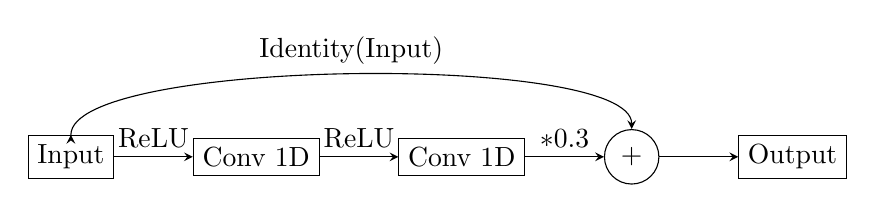
\begin{tikzpicture}
      \node[draw] (input) at (0, 0) {Input};
      \node[draw, right=of input] (conv1d1) {Conv 1D};
      \node[draw, right=of conv1d1] (conv1d2) {Conv 1D};
      \node[draw, circle, right=of conv1d2] (sum) {+};
      \node[draw, right=of sum] (output) {Output};
      \draw[-stealth] (input.east) -- (conv1d1.west) node[midway,above] {ReLU};
      \draw[-stealth] (conv1d1.east) -- (conv1d2.west) node[midway,above] {ReLU};
      \draw[-stealth] (conv1d2.east) -- (sum.west) node[midway,above] {$* 0.3$};
      \draw[-stealth] (sum.east) -- (output.west) node[midway,above] {};
      \draw[-stealth] (input.north) edge[out=90,in=90,looseness=0.35] 
      node[pos=0.3,midway,above] {Identity(Input)} (sum.north);
    \end{tikzpicture}
  \end{center}
  \caption{%
    \textquote{PassGAN} metodo neuroninio tinklo sluoksnių vieno likutinio bloko 
    sandara.
  }
  \label{plot:passganblock}
\end{figure}

Pilna neuroninių tinklų struktūrą -- generatoriaus ir diskriminatoriaus tinklų 
(modelių) -- pateikta priede \ref{plot:passganarch}.

\subsubsubsection{Pritaikymas slaptažodžių parinkimui}
Generatyviniai besivaržantys tinklai gali būti taikomi ir naujų slaptažodžių 
sintezei, taip parenkant naujus slaptažodžius. Iš apmokymo duomenų -- nutekintų 
slaptažodžių duomenų bazių -- generavimo modelis išmoksta slaptažodžių požymius 
pagal tai, ar generuojami slaptažodžiai suklasifikuoti kaip tikri ar ne tikri 
diskriminatoriaus modelio.

\subsubsubsection{Pastebėjimai}
\textquote{PassGAN} metodas parenka daugiau slaptažodžiu su didesniu kiekiu 
generuojamų slaptažodžių, t.y. kuo didesnis sugeneruotų slaptažodžių kiekis, tuo 
daugiau parenkamų slaptažodžių nežinomų slaptažodžių aibėje -- šio metodo 
moksliniame straipsnyje atliktas tyrimas parodo, kad modelis, apmokytas su $80$ 
\% \textquote{RockYou} nutekintos slaptažodžių duomenų bazės rinkinio 
slaptažodžių aibe, testuojamas su $20$ \% tos pačios duomenų bazės testavimo 
duomenų ir \textquote{Linkedin} duomenų aibėmis, parenka slaptažodžius kiekiais, 
pateiktais \ref{tab:passgan-original-results} lent., kurioje matyti, kad su kuo 
didesniu kiekiu sugeneruotų slaptažodžių, tuo didesnis yra parinktų slaptžodžių 
skaičius testavimo duomenų aibėje. Pastebėtina, kad iš $10^{10}$ sugeneruotų 
slaptažodžių, tik $21.5282$ \% sudaro unikalios reikšmės, t.y. $78.4718$ \% visų 
slaptažodžių yra dublikatai.

\begin{table}[hb]
  \centering
  \caption{%
    Slaptažodžių, sugeneruotų \textquote{PassGAN} metodu, apmokytų $80$ \% 
    \textquote{RockYou} duomenų ir sutampančių su \textquote{RockYou} testavimo 
    duomenų aibe \cite{PassGAN}.
  }
  \begin{tabular}{|c|c|c|}
    \hline \textbf{Slaptažodžių kiekis} & \textbf{Unikalūs slaptažodžiai} & 
    \textbf{Sutampančių slaptažodžių kiekis} \\
    \hline $10^4$ & 9738 & $0.005$ \% \\
    \hline $10^5$ & 94400 & $0.048$ \% \\
    \hline $10^6$ & 855972 & $0.381$ \% \\
    \hline $10^7$ & 7064483 & $2.038$ \% \\
    \hline $10^8$ & 52815412 & $6.726$ \% \\
    \hline $10^9$ & 356216832 & $15.094$ \% \\
    \hline $10^{10}$ & 2152819961 & $26.036$ \% \\
    \hline
  \end{tabular}
  \label{tab:passgan-original-results}
\end{table}

Atlikus analizę \textquote{PassGAN} metodo moksliniame straipsnyje pateiktų 
sugeneruotų slaptažodžių dublikatų skaičių, pateiktų
\ref{plot:passgan-original-duplicates} pav., nustatyta, kad didžioji dalis 
sugeneruotų unikalių slaptažodžių yra nuo $10^4$-$10^7$, toliau daugiau nei $50$ 
\% sudaro dublikatai.

\begin{figure}[!ht]
  \begin{center}
    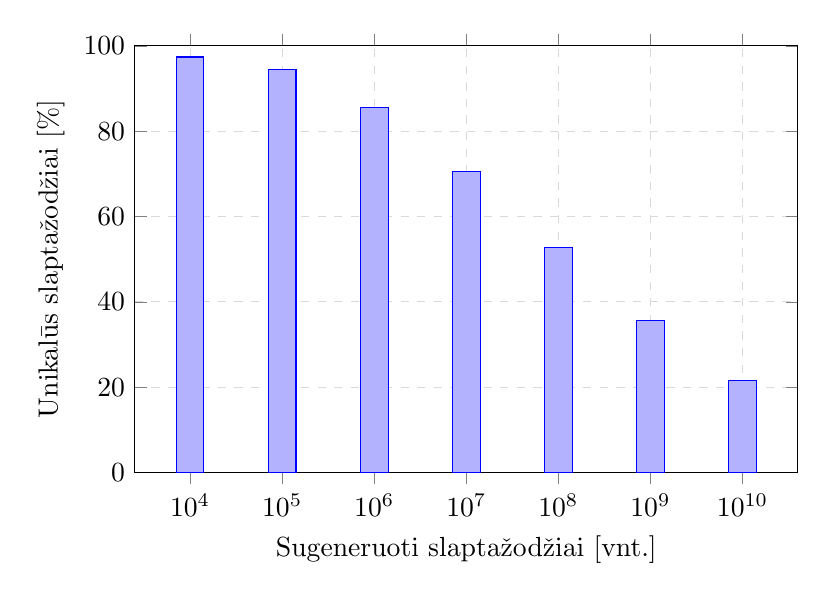
\begin{tikzpicture}
      \begin{axis}[
        ybar,
        xlabel={Sugeneruoti slaptažodžiai},
        ylabel={Unikalūs slaptažodžiai},
        x unit={vnt.},
        y unit={\%},
        ymin=0,
        ymax=100,
        xticklabels={,,$10^4$,$10^5$,$10^6$,$10^7$,$10^8$,$10^9$,$10^{10}$},
        grid=major,
        grid style={dashed,gray!30},
        width=10cm,
        height=7cm,
      ]
      \addplot coordinates {
        (1, 97.38)
        (2, 94.4)
        (3, 85.5972)
        (4, 70.64483)
        (5, 52.815412)
        (6, 35.621683)
        (7, 21.5282)
      };
      \end{axis}
    \end{tikzpicture}
  \end{center}
  \caption{%
    Unikalių slaptažodžių, sugeneruotų \textquote{PassGAN} metodu, kiekis.
  }
  \label{plot:passgan-original-duplicates}
\end{figure}

\subsubsection{\textquote{PCFG} metodas}
\subsubsubsection{Apie tikimybinius gramatikos taisyklių rinkinius}
\textquote{PCFG} (angl. \textquote{Probabilistic Context Free Grammar}) -- 
tikimybinis gramatikos taisyklių rinkinys, nurodantis, kaip kažkurį tai 
simbolį-reikšmę galima transformuoti į kitą simbolį. \textquote{PCFG} algoritmas 
yra pagrįstas gramatikos taisyklių rinkiniais (angl. \textquote{Context Free 
Grammar}) -- notacija, skirtą apibrėžti tam tikros formalios kalbos sintaksę, 
pvz. programinio kodo šaltinių failų analizei ir apdorojimui į simbolių grupių 
leksinį medį (kaip simbolių grupės yra susijusios su viena kita, ką jos 
reiškia). Tikimybiniai gramatikos taisyklių rinkiniai (angl. 
\textquote{Probabilistic Context Free Grammar}) yra tokie gramatikos taisyklių 
rinkiniai, kuriose kiekvienai simbolių grupei yra priskirta tikimybė. 
Tikimybiniai gramatikos taisyklių rinkiniai yra kilę iš kompiuterinės 
lingvistikos srities, skirta analizuoti ir modeliuoti natūralią kalbą -- 
simbolių grupių (pasikartojimo) tikimybės gali būti naudojamos kaip parametrai 
mašininio mokymosi modelyje, tačiau tikimybių reikšmės ypač priklauso nuo 
duomenų (kiekio, įvairovės), iš kurių jos yra išvestos.

\subsubsubsection{Pritaikymas slaptažodžių parinkimui}
\textquote{PCFG} metodą galima pritaikyti ir slaptažodžių gramatikos (formalios 
kalbos notacijos) nustatymui, ir, pagal šią gramatiką, parinkti naujus 
slaptažodžius. Naujų slaptažodžių parinkimui yra saugomos simbolių grupių 
reikšmės -- slaptažodžiai yra dalinami ir sugrupuojami į sujungtas skaitmenų, 
raidžių ir specialiųjų simbolių grupes, kurios yra įstatomos į slaptažodžio 
gramatiką parenkant naujus slaptažodžius.

\subsubsubsection{Algoritmo apžvalga} \label{sec:pcfgalg}
Slaptažodžių parinkimo strategijoje, \textquote{PCFG} algoritmas kiekvienam 
slaptažodžiui iš apmokymo duomenų rinkinio pirmiausia išveda gramatiką, t.y. 
simbolių grupės yra sugrupuojamos pagal tipą: skaitmenys, raidės, specialūs 
simboliai ir kartu užfiksuojami su konkrečių simbolių sekų bei pačios gramatikos 
pasikartojimų skaičiumi medžio pagrindo duomenų struktūroje (paprastai binarinis 
medis, angl. \textquote{Binary Tree}). Kai visi slaptažodžiai yra apdoroti į jų 
atitinkamas gramatikas, paskaičiuojami gramatikų ir simbolių grupių 
pasikartojimo dažniai -- kiek kartų gramatika ir ją sudarančios simbolių grupių 
reikšmės pasikartoja visoje apmokymo duomenų aibėje. Minėti dažniai yra 
naudojami parenkant naujus slaptažodžius -- pirmiausia parenkami slaptažodžiai, 
kurių gramatika ir gramatikoje esančių simbolių grupių dažniai yra didžiausi, 
tokiu būdu slaptažodžiai su aukščiausia tikimybe yra parenkami pirmi. Kitaip 
tariant, slaptažodžiai, kurių forma, struktūra ir skaitmenų, raidžių, specialių 
simbolių junginių grupės pasikartoja daugiausiai, sudaro šio metodo pirmąsias 
išvestis.
Viena gramatika \textquote{PCFG} algoritme gali būti panaudota kelis kartus 
parenkant slaptažodžius. \textquote{PCFG} algoritme yra išskiriami du tipai 
slaptažodžių -- preliminarūs (angl. \textquote{Pre-terminal}) ir galutiniai 
(angl. \textquote{Terminal}). Kiekvienas preliminarus slaptažodis yra parenkamas 
atsižvelgiant į jo ašies reikšmę, t.y. simbolių grupės, kuri buvo 
pakeista/transformuota parenkant šį slaptažodį, indeksas (pirminė ašies reikšmė 
parenkant pirmuosius preliminarius slaptažodžius yra lygi nuliui). Galutinių 
slaptažodžių parinkimo ir preliminarių slaptažodžių transformavimo taisyklės yra 
tokios:
\begin{enumerate}
  \item preliminariame slaptažodyje simbolių grupė gali būti keičiama tik jei 
    preliminaraus slaptažodžio ašies vertė yra mažesnė už grupės indeksą 
    slaptažodžio gramatikoje;
  \item preliminaraus slaptažodžio nauja ašis yra slaptažodyje pakeistos 
    simbolių grupės indeksas, skaičiuojant nuo 0;
  \item iš preliminaraus slaptažodžio yra parenkamas galutinis slaptažodis kai 
    yra pakeičiama viena ir tik viena simbolių grupė.
\end{enumerate}

Vadovaujantis aukščiau minėtomis taisyklėmis yra parenkami nauji galutiniai ir 
preliminarūs slaptažodžiai su transformuotomis simbolių grupėmis. Galutinis 
slaptažodis yra grąžinamas algoritmo, kai nebėra daugiau transformacijų, kurios 
galėtų būti su juo atliktos, o nauji preliminarūs slaptažodžiai, kuriems jau 
buvo atliktos transformacijos, yra grąžinami į algoritmo sąrašą tolesnėms 
transformacijoms.

Imant konkretų pavyzdį, tarkime metodas apdorojo slaptažodžių sąrašą ir sudarė 
sąrašą gramatikų ir raidžių, specialių simbolių, skaitmenų, bei jų pasikartojimo 
tikimybėmis. Šiam pavyzdžiui minėtas raidžių, specialių simbolių ir skaitmenų 
sąrašas pateiktas \ref{tab:pcfgvalues} lent.
\begin{table}[hb]
  \centering
  \caption{%
    Slaptažodžių kiekių augimas priklausant nuo slaptažodžio ilgio, 95 simbolių 
    aibėje (\textquote{ASCII} koduotėje).
  }
  \begin{tabular}{|c|c|c|}
    \hline \textbf{Gramatikos grupė} & \textbf{Reikšmė} & \textbf{Tikimybė} \\
    \hline A4 & pass & 0.8 \\
    \hline A3 & App & 0.75 \\
    \hline A3 & dSA & 0.74 \\
    \hline A3 & aOS & 0.72 \\
    \hline A2 & qw & 0.68 \\
    \hline S3 & \^\&* & 0.64 \\
    \hline S2 & !* & 0.55 \\
    \hline S2 & @@ & 0.48 \\
    \hline S2 & .( & 0.45 \\
    \hline S1 & \% & 0.36 \\
    \hline S1 & \$ & 0.3 \\
    \hline D3 & 123 & 0.25 \\
    \hline D2 & 33 & 0.25 \\
    \hline D2 & 47 & 0.24 \\
    \hline D2 & 29 & 0.12 \\
    \hline
  \end{tabular}
  \label{tab:pcfgvalues}
\end{table}
Tarkime, kad pirmoji (aukščiausios tikimybės) slaptažodžio gramatika yra 
\textquote{A3S2D2}, kurią galima skaityti taip -- slaptažodį sudaro trys raidės, 
du specialūs simboliai ir du skaitmenys. Ši gramatika buvo sugeneruota metodui 
išanalizavus slaptažodžius, kurių daugumą sudarė aukščiau minėta struktūra ir 
forma, neatsižvelgiant į kokios raidės, specialūs simboliai ir skaitmenys minėtą 
gramatiką sudarė. Inicijavus šią gramatiką išsaugotomis (sukauptomis) raidžių, 
specialių simbolių ir skaitmenų simbolių grupėmis (reiškiniais), kurie 
daugiausia pasikartoja tarp išanalizuotų slaptažodžių, galime gauti slaptažodį 
\textquote{App!*33}, kurio pradinė ašies reikšmė yra lygi nuliui. Parenkant 
pradines reikšmes pirminiams slaptažodžiams, pirmenybė skiriama reikšmėms su 
aukščiausia tikimybe (t.y. dažniausiai pasikartojo išanalizuotuose 
slaptažodžiuose). Atsižvelgiant į šio pradinio slaptažodžio ašies reikšmę (kuri 
yra lygi nuliui), galima atlikti tris transformacijas -- pakeisti grupes 
\textquote{A3}, \textquote{S2} ir \textquote{D2}, t.y. pakeisti kiekvieną 
simbolių grupę arba reiškinį vieną kartą, sugeneruojant 3 naujas šio 
slaptažodžio variacijas, po vieną kiekvienai transformacijai. Pakeitus grupę 
\textquote{A3}, ašies reikšmę -- nulį -- pakeičiame grupės indeksu -- nuliu 
(kadangi indeksą skaičiuojame nuo nulio), ir tai atlikus kitoms grupėms 
atitinkamai gauname jų ašies indeksus 1 ir 2. Taikant skyriuje \ref{sec:pcfgalg} 
pateiktas slaptažodžių transformavimo taisykles, atsižvelgiant į naujai 
sugeneruotų (transformuotų) 3 slaptažodžių ašies indeksus -- 0, 1 ir 2 -- galima 
toliau atlikti tokias transformacijas, kai šie minėti trys transformuoti 
slaptažodžiai bus išvesti:
\begin{itemize}
  \item iš pirmo transformuoto slaptažodžio, kurio ašies indeksas yra lygus 
    nuliui, išvesti 3 naujus transformuotus slaptažodžius, pakeitus 1-3 grupes;
  \item iš antro transformuoto slaptažodžio, kurio ašies indeksas yra lygus 
    vienam, išvesti 2 naujus transformuotus slaptažodžius, pakeitus 2-3 grupes;
  \item iš trečio transformuoto slaptažodžio, kurio ašies indeksas yra lygus 
    dviem, išvesti 1 naują transformuotą slaptažodį, pakeitus 3 grupę.
\end{itemize}

Grupių (reiškinių) pakeitimai yra atliekami tol, kol transformacijų ašies 
reikšmė nepasiekia paskutinės grupės, arba nepasibaigia simbolių grupės 
(reiškiniai), su kuriais būtų galima atlikti šiuos pakeitimus, žr. 
\ref{plot:pcfgtransforms} pav.

\begin{figure}
  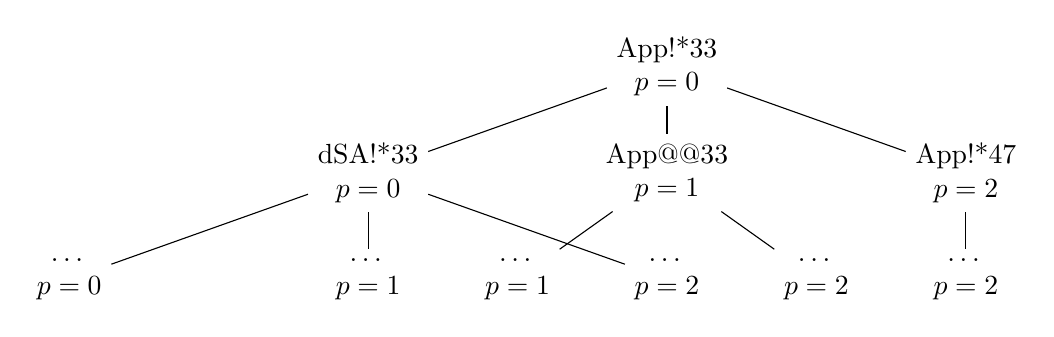
\begin{tikzpicture}[
    scale=0.9,
    every node/.style={scale=0.9},
    sibling distance=12em,
    every node/.style = {
      shape=rectangle,
      sharp corners,
      align=center
    }
  ]
    \node { App!*33 \\ $p=0$ }
      % Replace first group
      child { node { dSA!*33 \\ $p=0$ }
        child { node { \ldots \\ $p=0$ } }
        child { node { \ldots \\ $p=1$ } }
        child { node { \ldots \\ $p=2$ } }
      }
      % Replace second group
      child { node { App@@33 \\ $p=1$ }
        child { node { \ldots \\ $p=1$ } }
        child { node { \ldots \\ $p=2$ } }
      }
      % Replace third group
      child { node { App!*47 \\ $p=2$ }
        child { node { \ldots \\ $p=2$ } }
      };
  \end{tikzpicture}
  \caption{%
    Slaptažodžio \textquote{App!*33}, kurio gramatika \textquote{A3S2D2},
    transformacijų medis.
  }
  \label{plot:pcfgtransforms}
\end{figure}

\subsubsubsection{Pastebėjimai}
Algoritmas pabaigą pasiekia tada, kai gramatikos arba unikalios simbolių grupės 
pasibaigia ir/arba naujiems slaptažodžiams parinkti trūksta duomenų -- raidžių, 
skaitmenų ar specialių simbolių junginių. Parenkamų slaptažodžių bei gramatikų 
ir simbolių grupių kiekiai priklauso nuo apmokymo duomenų rinkinio dydžio -- yra 
svarbu pateikti ne didelį duomenų kiekį, bet duomenis, kuriose yra daug 
pasikartojančių reikšmių. Šios pasikartojančios reikšmės yra naudojamos 
tikimybių skaičiavimams ir turi įtaką, kokie slaptažodžiai bus parenkami 
slaptažodžių parinkimo proceso pradžioje.
Algoritmas slaptažodžius parinks tik tokius, kurių gramatikos buvo užfiksuotos 
apmokymui pateiktų slaptažodžių aibėje -- naujų gramatikų ir slaptažodžių formų 
nėra.

\section{Pagrindinė tiriamoji dalis}
\subsection{Etika}
Šis darbas buvo atliktas pagal Europos elgesio kodeksą mokslinių tyrimų etikos 
klausimais
(angl. \textquote{European Code of Conduct for Research Integrity}), paruoštą 
\textquote{European Federation of Academies of Sciences and Humanities} (ALLEA) 
organizacijos. Kadangi nutekintos duomenų bazės yra sudarytos iš galimų 
vartotojų asmeninės informacijos (pvz. vardas, pavardė, elektroninis pašto 
adresas), visa informacija buvo saugiai laikoma ir tvarkoma. Asmens duomenų 
atskleidimo galimybės buvo mažinamos įgyvendinant griežtas saugumo priemones, ir 
nutekinti slaptažodžiai nebuvo testuojami su tikromis internetinių paslaugų 
vartotojų paskyromis. Darbe atskleidžiami tik patys dažniausiai pasikartojantys 
slaptažodžiai, jų sudėtingumas ir struktūra. Slaptažodžiai, kurie galėtų būti 
naudojami vartotojų identifikacijai, nebuvo atskleisti. Vartotojų asmeninė 
informacija yra nepateikta.

\subsection{Nutekintų slaptažodžių duomenų bazių analizė} \label{sec:db-analize}
Šiame darbe naudojamos dvi nutekintų slaptažodžių duomenų bazės, atvirai 
prieinamos viešais šaltiniais -- \textquote{RockYou} \cite{RockYou} ir 
\textquote{Linkedin} \cite{Linkedin}. Dešimt dažniausiai pasikartojančių 
slaptažodžių duomenų bazėje \textquote{RockYou} yra pateikti \ref{tab:rockyou10} 
lentelėje, o duomenų bazėje \textquote{Linkedin} -- \ref{tab:linkedin10} 
lentelėje. Turimą \textquote{RockYou} nutekintą slaptažodžių duomenų bazę sudaro 
iš viso $32603388$ įrašai, iš kurių $14283864$ ($43.81 \%$ visų įrašų) 
slaptažodžiai yra unikalūs. Turimą \textquote{Linkedin} nutekintą slaptažodžių 
duomenų bazę sudaro iš viso $8616484$ įrašai, iš kurių $4878546$ ($56.61 \%$ 
visų įrašų) yra unikalūs ir su \textquote{RockYou} įrašais sutampa $664704$ (iš 
viso $2.04 \%$ visų \textquote{RockYou} irašų). Pastebėtina, kad naudojama ne 
pilna \textquote{Linkedin} nutekinta slaptažodžių duomenų bazė, o tik jos dalis 
-- $10.79$ \% visos $2.91$ GB nutekintos slaptažodžių duomenų bazės, jau 
parinkti slaptažodžiai.

% If unsorted and unnumbered, use command:
% $ sort DB.txt | uniq -c | sort -nr | head -n 10
\begin{table}[hb]
  \centering
  \caption{%
    Duomenų rinkinio \textquote{RockYou} 10 dažniausiai pasikartojančių 
    slaptažodžių.
  }
  \begin{tabular}{|c|c|}
    \hline \textbf{Kiekis} & \textbf{Slaptažodis} \\
    \hline 290729 & 123456 \\
    \hline 79076 & 12345 \\
    \hline 76789 & 123456789 \\
    \hline 59462 & password \\
    \hline 49952 & iloveyou \\
    \hline 33291 & princess \\
    \hline 21725 & 1234567 \\
    \hline 20901 & rockyou \\
    \hline 20553 & 12345678 \\
    \hline 16648 & abc123 \\
    \hline
  \end{tabular}
  \label{tab:rockyou10}
\end{table}

\ref{tab:rockyou10} lentelėje pateikti slaptažodžiai daugiausia sudaryti iš 
bendrinių daiktavardžių, paprastų skaičių ir raidžių sekų.

\begin{table}[ht]
  \centering
  \caption{%
    Duomenų rinkinio \textquote{Linkedin} 10 dažniausiai pasikartojančių 
    slaptažodžių.
  }
  \begin{tabular}{|c|c|}
    \hline \textbf{Kiekis} & \textbf{Slaptažodis} \\
    \hline 3 & YoshitakaKatayama1 \\
    \hline 3 & y0m@r3352 \\
    \hline 3 & xingopenBC \\
    \hline 3 & wustlukelib \\
    \hline 3 & Viktor27MAJ \\
    \hline 3 & VidSofija2011 \\
    \hline 3 & ttphung_2001 \\
    \hline 3 & toque99can \\
    \hline 3 & tklC2007* \\
    \hline 3 & Tigerman13101905 \\
    \hline
  \end{tabular}
  \label{tab:linkedin10}
\end{table}

\ref{tab:rockyou10}, \ref{tab:linkedin10} lentelėse pateikti dažniausi vartotojų 
slaptažodžiai yra daugiausia sudaryti iš lotyniškos abėcėlės raidžių bei 
skaitmenų. Paminėtina, kad naudojama \textquote{Linkedin} nutekinta slaptažodžių 
duomenų bazė yra deduplikuota -- pašalinti pasikartojantys įrašai.

\begin{figure}[!ht]
  \begin{center}
    \begin{tikzpicture}
      \begin{axis}[
        xlabel={Ilgis},
        ylabel={Kiekis},
        x unit={simboliai},
        y unit={vnt.},
        grid=major,
        grid style={dashed,gray!30},
        width=10cm,
        height=7cm,
      ]
      \addplot
        table[x=length, y=count, col sep=comma, comment 
        chars={~}]{rockyou_length.csv};
      \end{axis}
    \end{tikzpicture}
  \end{center}
  \caption{%
    Nutekintos slaptažodžių duomenų bazės \textquote{RockYou} įrašų ilgiai.
  }
  \label{plot:rockyoulength}
\end{figure}

\begin{figure}[!ht]
  \begin{center}
    \begin{tikzpicture}
      \begin{axis}[
        xlabel={Ilgis},
        ylabel={Kiekis},
        x unit={simboliai},
        y unit={vnt.},
        grid=major,
        grid style={dashed,gray!30},
        width=10cm,
        height=7cm,
      ]
      \addplot
        table[x=length, y=count, col sep=comma, comment 
      chars={~}]{linkedin_length.csv};
      \end{axis}
    \end{tikzpicture}
  \end{center}
  \caption{%
    Nutekintos slaptažodžių duomenų bazės \textquote{Linkedin} įrašų ilgiai.
  }
  \label{plot:linkedinlength}
\end{figure}

Atlikta nutekintų slaptažodžių duomenų bazių įrašų ilgių analizė (žr. 
\ref{plot:rockyoulength}, \ref{plot:linkedinlength} pav.) parodo, kad daugiausia 
vartotojų sukurtų slaptažodžių yra tarp 5-10 simbolių ilgio (slaptažodžiai, 
ilgesni nei 16 simbolių, buvo atmesti pateiktuose vizualizacijose, kadangi jų 
kiekiai buvo per maži).

\subsection{Eksperimentuose taikoma strategija} \label{sec:strategy}
Su pasirinktu automatizuoto slaptažodžių parinkimo metodu ir naudojant jo 
realizacijos moksliniame straipsnyje apibrėžtus rekomenduojamus parametrus bus 
apmokytas modelis su $80$ \% duomenų nuo visos pasirinktos nutekintos 
slaptažodžių duomenų bazės įrašų aibės, likusieji $20$ \% bus naudojami 
testavimui. Nutekintoms slaptažodžių duomenų bazėms, kurios minėtos ir 
analizuotos \ref{sec:db-analize} skyriuje, bus naudojamos modelių apmokymui. 
Siekiant įvertinti automatizuoto slaptažodžio parinkimo metodo efektyvumą, bus 
generuojami tarp $10^{4}$ ir $10^{10}$ slaptažodžių, kurie bus testuojami su 
$20$ \% įrašų iš apmokymui naudojamos duomenų bazės testavimo duomenų aibės, ir 
su kita, anksčiau modelio nematyta nutekinta slaptažodžių duomenų baze. 
Generuojant mažiau, nei $10^{4}$ slaptažodžių, \textquote{PassGAN} metodas 
nesugeneravo slaptžodžių, o \textquote{PCFG} -- turėjo mažesnį, nei $1$ \% 
tikslumą, dėl to nebus lyginami mažesni, nei $10^{4}$, slaptažodžių kandidatų 
sąrašai. Modelio apmokymas vyks su \textquote{RockYou} nutekinta slaptažodžių 
duomenų baze dėl joje esančių didelių (unikalių) slaptažodžių kiekių, palyginus 
su naudojama \textquote{Linkedin} nutekinta slaptažodžių duomenų baze.

Testavimas bus atliktas palyginant sugeneruotą slaptažodžių sąrašą su testavimo 
duomenų aibe \textquote{Linux} pagrindo operacinės sistemos programų paketo 
\textquote{Coreutils - GNU core utilities} įrankių \textquote{sort}, 
\textquote{uniq}, \textquote{split}, \textquote{wc}, \textquote{comm}, 
\textquote{gawk} pagalba \cite{Coreutils}. Sugeneruotas slaptažodžių sąrašas bus 
išrikiuotas, tarp sugeneruotos ir testavimo duomenų aibių bus išskirti bendri 
įrašai, suskaičiuotas įrašų skaičius ir paskaičiuota, kokią dalį sudaro bendrų 
įrašų skaičius testavimo duomenų aibės.

Slaptažodžių, sutampančių su $20$ \% testavimo duomenų aibės slaptažodžiais ir 
su kitoje nutekintoje duomenų bazėje esančiais slaptažodžiais, kiekis bus 
fiksuojamas kiekvienam sugeneruotų slaptažodžių rinkiniui.

Visi eksperimentai atlikti su operacinių sistemų \textquote{Microsoft Windows 
10} (versija \textit{21H2}), \textquote{Linux} distribucijos \textquote{NixOS} 
(versija \textit{22.05}, \textquote{Linux} branduolio versija 
\textit{5.10.16.3-microsoft-standard-WSL2}) pagalba, naudojant 64 GB 
operatyviosios atminties, 6 branduolių 3.2 GHz \textquote{Intel Core i7-8700} 
procesorių ir 3 GB atminties \textquote{NVIDIA GeForce GTX 1060} vaizdo plokšte.

\subsection{\textquote{PassGAN} eksperimentų serija}
Šioje dalyje atliekami eksperimentai su \textquote{PassGAN} metodo realizacija 
\cite{PassGAN:impl}, generuojant slaptažodžių sąrašus pagal \ref{sec:strategy} 
skyriuje aprašytą strategiją.

\subsubsection{Eksperimentas su \textquote{RockYou} rinkiniu} % --------------- 
\label{sec:pgrockyou}
\begin{table}[hb]
  \centering
  \caption{%
    \textquote{PassGAN} metodu apmokyto modelio sugeneruotų slaptažodžių, 
    sutampančių su $20$ \% \textquote{RockYou} duomenų rinkinio testavimo
    slaptažodžių aibe, dalis.
  }
  \begin{tabular}{|c|c|c|c|}
    \hline \textbf{Kiekis} & \textbf{Unikalūs} & \textbf{Sutampantys} & 
    \textbf{Sutampantys (\%)} \\
    \hline $10^4$ & 9040 & 1034 & $0.028584$ \% \\
    \hline $10^5$ & 95295 & 9224 & $0.254988$ \% \\
    \hline $10^6$ & 885174 & 54453 & $1.505298$ \% \\
    \hline $10^7$ & 7489667 & 191192 & $5.285309$ \% \\
    \hline $10^8$ & 57162878 & 447070 & $12.358798$ \% \\
    \hline $10^9$ & 390305149 & 788802 & $21.805633$ \% \\
    \hline $10^{10}$ & 2379342789 & 1162151 & $32.126489$ \% \\
    \hline
  \end{tabular}
  \label{tab:passgan-rockyou-results}
\end{table}
Apmokytas modelis su $80$ \% \textquote{RockYou} duomenų rinkiniu ir, 
pirmiausia, atliktas testavimas su $20$ \% to paties duomenų rinkinio testavimo 
duomenų aibe, kurio rezultatai pateikti \ref{tab:passgan-rockyou-results} lent.

Nustatyta, kad \ref{tab:passgan-rockyou-results} lent. pateikti duomenys rodo, 
kad apmokyto modelio parinktų slaptažodžių skaičiai panašūs į 
\textquote{PassGAN} metodo mokslinio straipsnio autoriaus rezultatus, pateiktus 
\ref{tab:passgan-original-results} lent.

\begin{figure}[!ht]
  \begin{center}
    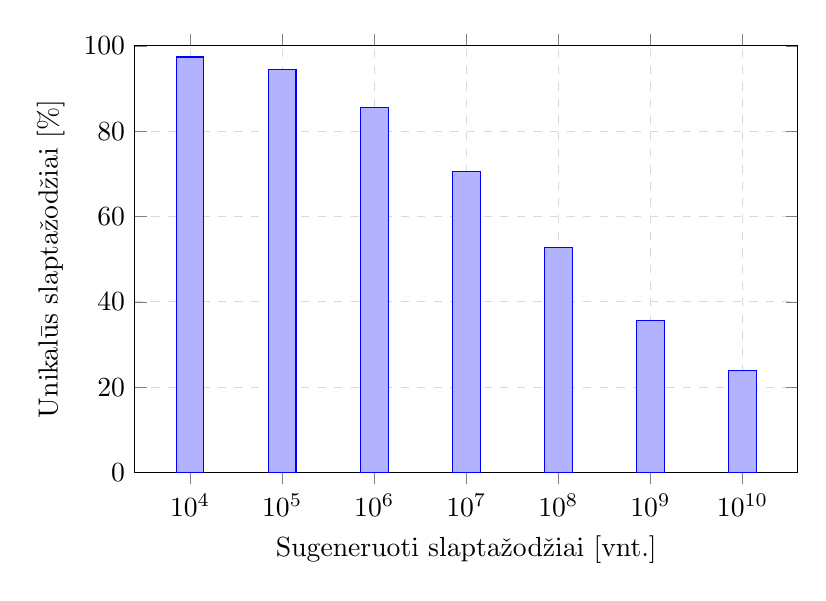
\begin{tikzpicture}
      \begin{axis}[
        ybar,
        xlabel={Sugeneruoti slaptažodžiai},
        ylabel={Unikalūs slaptažodžiai},
        x unit={vnt.},
        y unit={\%},
        ymin=0,
        ymax=100,
        xticklabels={,,$10^4$,$10^5$,$10^6$,$10^7$,$10^8$,$10^9$,$10^{10}$},
        grid=major,
        grid style={dashed,gray!30},
        width=10cm,
        height=7cm,
      ]
      \addplot coordinates {
        (1, 97.38)
        (2, 94.4)
        (3, 85.5972)
        (4, 70.64483)
        (5, 52.815412)
        (6, 35.621683)
        (7, 23.793428)
      };
      \end{axis}
    \end{tikzpicture}
  \end{center}
  \caption{%
    Unikalių slaptažodžių, sugeneruotų \textquote{PassGAN} metodu, dalis.
  }
  \label{plot:passgan-rockyou-duplicates}
\end{figure}
Atlikus analizę \textquote{PassGAN} metodu sugeneruotų slaptažodžių dublikatų 
dalies, nustatyta, kad yra panaši dublikuotų slaptažodžių dalis, kaip pateikta 
\ref{plot:passgan-original-duplicates} pav. \textquote{PassGAN} autorių 
pasiektuose rezultatuose.
\begin{figure}[!ht]
  \begin{center}
    \begin{tikzpicture}
      \begin{axis}[
        xlabel={Sugeneruoti slaptažodžiai},
        ylabel={Sutampantys slaptažodžiai},
        x unit={vnt.},
        y unit={\%},
        ymin=0,
        ymax=100,
        xticklabels={,,$10^4$,$10^5$,$10^6$,$10^7$,$10^8$,$10^9$,$10^{10}$},
        grid=major,
        grid style={dashed,gray!30},
        width=10cm,
        height=7cm,
      ]
      \addplot coordinates {
        (1, 0.028584)
        (2, 0.254988)
        (3, 1.505298)
        (4, 5.285309)
        (5, 12.358798)
        (6, 21.805633)
        (7, 32.126489)
      };
      \addplot coordinates {
        (1, 0.005)
        (2, 0.048)
        (3, 0.381)
        (4, 2.038)
        (5, 6.726)
        (6, 15.094)
        (7, 26.036)
      };
      \legend{
        Mūsų rezultatai,
        Straipsnio autorių rezultatai
      }
      \end{axis}
    \end{tikzpicture}
  \end{center}
  \caption{%
    \textquote{PassGAN} metodu apmokyto modelio sugeneruotų slaptažodžių, 
    sutampančių su $20$ \% \textquote{RockYou} duomenų rinkinio testavimo
    slaptažodžių aibe, dalis, palyginus su \textquote{PassGAN} straipsnio 
    autorių skelbiamais rezultatais.
  }
  \label{plot:passgan-rockyou-comparison}
\end{figure}
Toliau atliktas palyginimas su \textquote{PassGAN} metodo autoriaus gautais 
rezultatais su tą pačia nutekinta slaptažodžių duomenų baze -- 
\textquote{RockYou} ($80$ \% slaptažodžių modelio apmokymui, likusieji $20$ \% 
testavimui) -- ir šiame darbe apmokyto modelio rezultatais, žr. 
\ref{plot:passgan-rockyou-comparison} pav.

Įvertinus \ref{plot:passgan-rockyou-comparison} pav. pateiktą informaciją, 
nustatyta, kad iki $10^8$ sugeneruotų slaptažodžių, slaptažodžių kiekis, 
sutampantis su testavimo duomenų aibe, sutampa ($1$ \% tikslumu), o didesniems 
generuojamų slaptažodžių kiekiams -- šiame darbe apmokytu modeliu maždaug 
$3$-$6$ \% daugiauslaptažodžių parenka. Toks slaptažodžių parinkimo tikslumo 
padidėjimas yra priskiriamas nutekintos slaptažodžių duomenų bazės 
\textquote{RockYou} išmaišymui prieš padalinant į apmokymo ir testavimo aibes. 
Slaptažodžiai, su kuriais buvo testuojamas modelis aukščiau minėtame 
straipsnyje, galimai pateko į apmokymo duomenų aibę šiame darbe, todėl parinkimo 
tikslumas neryškiai skiriasi (šiame darbe mokėsi iš kitų slaptažodžių, negu 
kokie buvo naudojami mokymui straipsnyje, tačiau tai nustatyti reikėtų daugiau 
informacijos apie duomenų rinkinio apdorojimą).

\subsubsection{Eksperimentas su \textquote{Linkedin} rinkiniu} % ---------------
\begin{table}[hb]
  \centering
  \caption{%
    \textquote{PassGAN} metodu apmokyto modelio sugeneruotų slaptažodžių, 
    sutampančių su visa \textquote{Linkedin} duomenų rinkinio testavimo
    slaptažodžių aibe, dalis.
  }
  \begin{tabular}{|c|c|c|c|}
    \hline \textbf{Kiekis} & \textbf{Unikalūs} & \textbf{Sutampantys} & 
    \textbf{Sutampantys (\%)} \\
    \hline $10^4$ & 9040 & 570 & $0.011684$ \% \\
    \hline $10^5$ & 95295 & 5063 & $0.103781$ \% \\
    \hline $10^6$ & 885174 & 29694 & $0.608665$\% \\
    \hline $10^7$ & 7489667 & 108965 & $2.233145$ \% \\
    \hline $10^8$ & 57162878 & 272536 & $5.586419$ \% \\
    \hline $10^9$ & 390305149 & 515889 & $10.574647$ \% \\
    \hline $10^{10}$ & 2379342789 & 813834 & $16.681897$ \% \\
    \hline
  \end{tabular}
  \label{tab:passgan-linkedin-results}
\end{table}

\begin{figure}[!ht]
  \begin{center}
    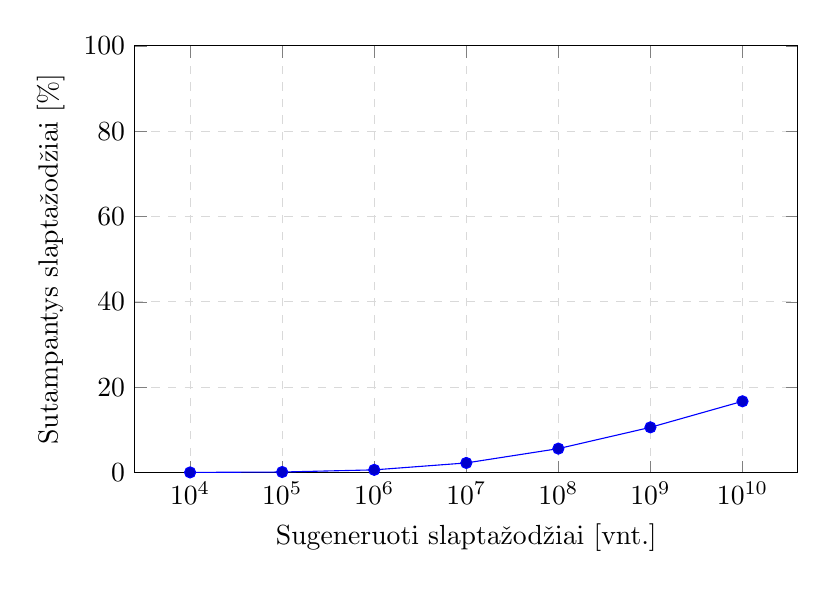
\begin{tikzpicture}
      \begin{axis}[
        xlabel={Sugeneruoti slaptažodžiai},
        ylabel={Sutampantys slaptažodžiai},
        x unit={vnt.},
        y unit={\%},
        ymin=0,
        ymax=100,
        xticklabels={,,$10^4$,$10^5$,$10^6$,$10^7$,$10^8$,$10^9$,$10^{10}$},
        grid=major,
        grid style={dashed,gray!30},
        width=10cm,
        height=7cm,
      ]
      \addplot coordinates {
        (1, 0.011684)
        (2, 0.103781)
        (3, 0.608665)
        (4, 2.233145)
        (5, 5.586419)
        (6, 10.574647)
        (7, 16.681897)
      };
      \end{axis}
    \end{tikzpicture}
  \end{center}
  \caption{%
    \textquote{PassGAN} metodu apmokyto modelio sugeneruotų slaptažodžių, 
    sutampančių su visa \textquote{Linkedin} duomenų rinkinio testavimo
    slaptažodžių aibe, dalis.
  }
  \label{plot:passgan-linkedin-results}
\end{figure}
\ref{sec:pgrockyou} skyriuje apmokytas modelis su $80$ \% \textquote{RockYou} 
duomenų rinkiniu yra toliau testuojamas su visa \textquote{Linkedin} duomenų 
rinkinio slaptažodžių aibe, žr. \ref{tab:passgan-linkedin-results} lent., 
\ref{plot:passgan-linkedin-results} pav. Palyginus šiuos rezultatus su 
\ref{sec:pgrockyou} skyriaus rezultatais, parenkama maždaug per pus mažiau 
slaptažodžių anksčiau nematytoje slaptažodžių duomenų bazėje -- tai gali nulemti 
kitokios, anksčiau nematytos slaptažodžių formos, požymiai, kurie nebuvo arba 
kurių neužteko apmokymo duomenų bazės slaptažodžiuose.

\subsection{\textquote{PCFG} eksperimentų serija}
Šioje dalyje atliekami eksperimentai su \textquote{PCFG} metodo realizacija 
\cite{PCFG:impl}, generuojant slaptažodžių sąrašus pagal \ref{sec:strategy} 
skyriuje aprašyta strategija.

\subsubsection{Eksperimentas su \textquote{RockYou} rinkiniu} % ---------------
\label{sec:pgpcfg}
\begin{table}[hb]
  \centering
  \caption{%
    \textquote{PCFG} metodu apmokyto modelio sugeneruotų slaptažodžių, 
    sutampančių su $20$ \% \textquote{RockYou} duomenų rinkinio testavimo
    slaptažodžių aibe, dalis.
  }
  \begin{tabular}{|c|c|c|c|}
    \hline \textbf{Kiekis} & \textbf{Unikalūs} & \textbf{Sutampantys} & 
    \textbf{Sutampantys (\%)} \\
    \hline $10^4$ & 9997 & 9958 & $0.275279$ \% \\
    \hline $10^5$ & 99952 & 97583 & $2.697583$ \% \\
    \hline $10^6$ & 997955 & 549337 & $15.185866$ \% \\
    \hline $10^7$ & 9984845 & 1160517 & $32.081319$ \% \\
    \hline $10^8$ & 99822373 & 1622905 & $44.863567$ \% \\
    \hline $10^9$ & 997519248 & 1966591 & $54.364419$ \% \\
    % \hline $10^{10}$ & 9804626984 & 632609 & $17.487836$ \% \\
    \hline $10^{10}$ & 9804626984 & 2071111 & $57.253791$ \% \\
    \hline
  \end{tabular}
  \label{tab:pcfg-rockyou-results}
\end{table}
Apmokytas modelis su $80$ \% \textquote{RockYou} duomenų rinkiniu ir, 
pirmiausia, atliktas testavimas su $20$ \% to paties duomenų rinkinio testavimo 
duomenų aibe, kurio rezultatai rezultatai pateikti 
\ref{tab:pcfg-rockyou-results} lent.

\begin{figure}[!ht]
  \begin{center}
    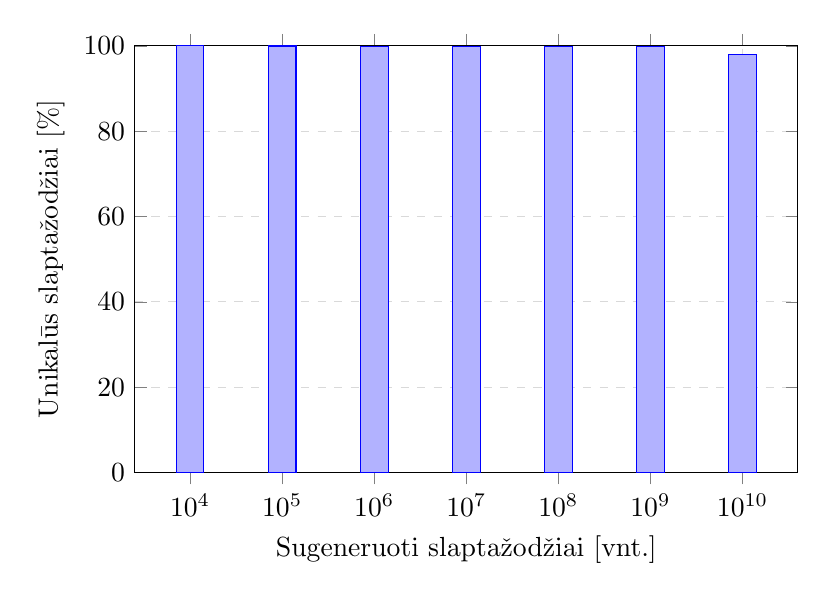
\begin{tikzpicture}
      \begin{axis}[
        ybar,
        xlabel={Sugeneruoti slaptažodžiai},
        ylabel={Unikalūs slaptažodžiai},
        x unit={vnt.},
        y unit={\%},
        ymin=0,
        ymax=100,
        xticklabels={,,$10^4$,$10^5$,$10^6$,$10^7$,$10^8$,$10^9$,$10^{10}$},
        grid=major,
        grid style={dashed,gray!30},
        width=10cm,
        height=7cm,
      ]
      \addplot coordinates {
        (1, 99.97)
        (2, 99.952)
        (3, 99.7955)
        (4, 99.84845)
        (5, 99.822373)
        (6, 99.751925)
        (7, 98.04627)
      };
      \end{axis}
    \end{tikzpicture}
  \end{center}
  \caption{%
    Unikalių slaptažodžių, sugeneruotų \textquote{PCFG} metodu, dalis.
  }
  \label{plot:pcfg-rockyou-duplicates}
\end{figure}
Atlikus analizę \textquote{PCFG} metodu sugeneruotų slaptažodžių dublikatų 
dalies, nustatyta, kad visuose sugeneruotuose $10^4$-$10^{10}$ slaptažodžių 
sąrašuose yra beveik visi unikalūs slaptažodžiai.

\begin{figure}[!ht]
  \begin{center}
    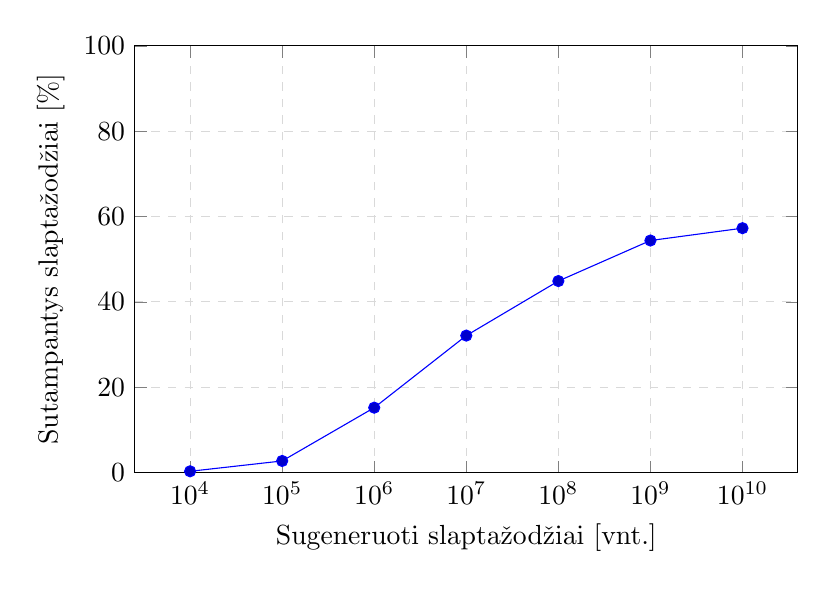
\begin{tikzpicture}
      \begin{axis}[
        xlabel={Sugeneruoti slaptažodžiai},
        ylabel={Sutampantys slaptažodžiai},
        x unit={vnt.},
        y unit={\%},
        ymin=0,
        ymax=100,
        xticklabels={,,$10^4$,$10^5$,$10^6$,$10^7$,$10^8$,$10^9$,$10^{10}$},
        grid=major,
        grid style={dashed,gray!30},
        width=10cm,
        height=7cm,
      ]
      \addplot coordinates {
        (1, 0.275279)
        (2, 2.697583)
        (3, 15.185866)
        (4, 32.081319)
        (5, 44.863567)
        (6, 54.364419)
        % (7, 17.487836)
        (7, 57.253791)
      };
      \end{axis}
    \end{tikzpicture}
  \end{center}
  \caption{%
    \textquote{PCFG} metodu apmokyto modelio sugeneruotų slaptažodžių, 
    sutampančių su $20$ \% \textquote{RockYou} duomenų rinkinio testavimo
    slaptažodžių aibe, dalis.
  }
  \label{plot:pcfg-rockyou-results}
\end{figure}
Pagal \ref{tab:pcfg-rockyou-results} lent. ir \ref{plot:pcfg-rockyou-results} 
pav. duomenis, nustatyta, kad geriausi rezultatai -- tarp $15$-$54$ \% -- buvo 
pasiekti $10^4$-$10^9$ sugeneruotų slaptažodžių aibėse. Pagal \textquote{PCFG} 
metodo ypatybes, yra galimybė, kad generuojant jau $10^{10}$ slaptažodžių 
sąrašą, geriausios reikšmės (slaptažodžiai su didžiausia tikimybe) buvo 
išnaudotos, parinktos, ir liko visos žemesnių tikimybių reikšmės, kurios jau 
nebepatenka į testavimo duomenų aibę.

\subsubsection{Eksperimentas su \textquote{Linkedin} rinkiniu} % ---------------
\begin{table}[ht]
  \centering
  \caption{%
    \textquote{PCFG} metodu apmokyto modelio sugeneruotų slaptažodžių, 
    sutampančių su visa \textquote{Linkedin} duomenų rinkinio testavimo
    slaptažodžių aibe, dalis.
  }
  \begin{tabular}{|c|c|c|c|}
    \hline \textbf{Kiekis} & \textbf{Unikalūs} & \textbf{Sutampantys} & 
    \textbf{Sutampantys (\%)} \\
    \hline $10^4$ & 9997 & 8681 & $0.177942$ \% \\
    \hline $10^5$ & 99952 & 65646 & $1.345606$ \% \\
    \hline $10^6$ & 997955 & 312668 & $6.409041$ \% \\
    \hline $10^7$ & 9984845 & 691975 & $14.184042$ \% \\
    \hline $10^8$ & 99822373 & 1155333 & $23.681913$ \% \\
    \hline $10^9$ & 997519248 & 1580818 & $32.403466$ \% \\ 
    % \hline $10^{10}$ & 9804626984 & 811776 & $16.639712$ \% \\
    \hline $10^{10}$ & 9804626984 & 1681782 & $34.473021$ \% \\
    \hline
  \end{tabular}
  \label{tab:pcfg-linkedin-results}
\end{table}

\begin{figure}[ht]
  \begin{center}
    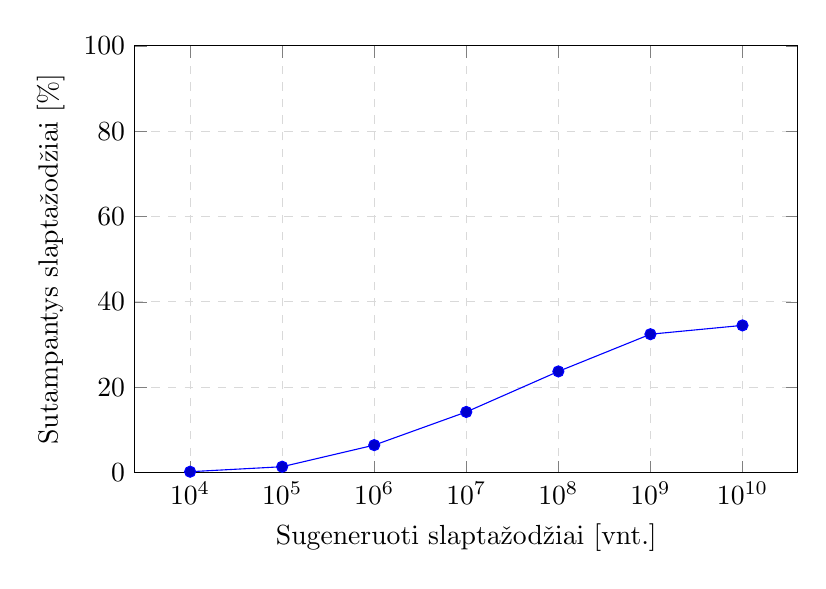
\begin{tikzpicture}
      \begin{axis}[
        xlabel={Sugeneruoti slaptažodžiai},
        ylabel={Sutampantys slaptažodžiai},
        x unit={vnt.},
        y unit={\%},
        ymin=0,
        ymax=100,
        xticklabels={,,$10^4$,$10^5$,$10^6$,$10^7$,$10^8$,$10^9$,$10^{10}$},
        grid=major,
        grid style={dashed,gray!30},
        width=10cm,
        height=7cm,
      ]
      \addplot coordinates {
        (1, 0.177942)
        (2, 1.345606)
        (3, 6.409041)
        (4, 14.184042)
        (5, 23.681913)
        (6, 32.403466)
        (7, 34.473021)
      };
      \end{axis}
    \end{tikzpicture}
  \end{center}
  \caption{%
    \textquote{PCFG} metodu apmokyto modelio sugeneruotų slaptažodžių, 
    sutampančių su visa \textquote{Linkedin} duomenų rinkinio testavimo
    slaptažodžių aibe, dalis.
  }
  \label{plot:pcfg-linkedin-results}
\end{figure}
\ref{sec:pgpcfg} skyriuje apmokytas modelis su $80$ \% \textquote{RockYou} 
duomenų rinkiniu yra toliau testuojamas su visa \textquote{Linkedin} duomenų 
rinkinio slaptažodžių aibe, žr. \ref{tab:passgan-linkedin-results} lent., 
\ref{plot:passgan-linkedin-results} pav. Įvertinus šiuos rezultatus, nustatyta, 
kad panašiai kaip su \textquote{PassGAN} metodu, parenkamų slaptažodžių skaičius 
(parinkimo tikslumas) nukrenta testuojant su anksčiau nematyta nutekinta 
slaptažodžių duomenų baze \textquote{Linkedin}.

\subsection{Eksperimentų rezultatų apžvalga}
Šioje dalyje su \textquote{PassGAN} ir \textquote{PCFG} metodais atliktų
eksperimentų rezultatai yra palyginami ir įvertinami. Diagramos, pateiktos 
\ref{plot:passgan-rockyou-comparison}, \ref{plot:passgan-linkedin-results}, 
\ref{plot:pcfg-rockyou-results}, \ref{plot:pcfg-linkedin-results} pav., yra 
apjungtos patogesnei rezultatų peržiūrai abiems metodams į 
\ref{plot:passgan-pcfg-comparison} pav.
\begin{figure}[H]
  \centering
  \begin{subfigure}{.5\textwidth}
    \centering
    \begin{tikzpicture}
      \begin{axis}[
        xlabel={Sugeneruoti slaptažodžiai},
        ylabel={Sutampantys slaptažodžiai},
        x unit={vnt.},
        y unit={\%},
        ymin=0,
        ymax=100,
        xticklabels={,,$10^4$,$10^5$,$10^6$,$10^7$,$10^8$,$10^9$,$10^{10}$},
        grid=major,
        grid style={dashed,gray!30},
        height=7cm,
      ]
      \addplot coordinates {
        (1, 0.028584)
        (2, 0.254988)
        (3, 1.505298)
        (4, 5.285309)
        (5, 12.358798)
        (6, 21.805633)
        (7, 32.126489)
      };
      \addplot coordinates {
        (1, 0.275279)
        (2, 2.697583)
        (3, 15.185866)
        (4, 32.081319)
        (5, 44.863567)
        (6, 54.364419)
        (7, 57.253791)
      };
      \legend{
        \textquote{PassGAN} metodas,
        \textquote{PCFG} metodas
      }
      \end{axis}
    \end{tikzpicture}
    \caption{Testuojamas modelis su $20$ \% \textquote{RockYou} duomenų 
    rinkiniu.}
    \label{plot:passgan-pcfg-rockyou-comparison}
  \end{subfigure}%
  \hfill
  \begin{subfigure}{.5\textwidth}
    \centering
    \begin{tikzpicture}
      \begin{axis}[
        xlabel={Sugeneruoti slaptažodžiai},
        ylabel={Sutampantys slaptažodžiai},
        x unit={vnt.},
        y unit={\%},
        ymin=0,
        ymax=100,
        xticklabels={,,$10^4$,$10^5$,$10^6$,$10^7$,$10^8$,$10^9$,$10^{10}$},
        grid=major,
        grid style={dashed,gray!30},
        height=7cm,
      ]
      \addplot coordinates {
        (1, 0.011684)
        (2, 0.103781)
        (3, 0.608665)
        (4, 2.233145)
        (5, 5.586419)
        (6, 10.574647)
        (7, 16.681897)
      };
      \addplot coordinates {
        (1, 0.177942)
        (2, 1.345606)
        (3, 6.409041)
        (4, 14.184042)
        (5, 23.681913)
        (6, 32.403466)
        (7, 34.473021)
      };
      \legend{
        \textquote{PassGAN} metodas,
        \textquote{PCFG} metodas
      }
      \end{axis}
    \end{tikzpicture}
    \caption{Testuojamas modelis su visu \textquote{Linkedin} duomenų rinkiniu.}
    \label{plot:passgan-pcfg-linkedin-comparison}
  \end{subfigure}
  \caption{%
    Parinkti slaptažodžiai tarp \textquote{PassGAN} ir \textquote{PCFG} metodo 
    modelių, apmokytų su $80$ \% \textquote{RockYou} nutekintos slaptažodžių 
    duomenų bazės įrašais
  }
  \label{plot:passgan-pcfg-comparison}
\end{figure}%
Palyginus \ref{plot:passgan-pcfg-rockyou-comparison} ir 
\ref{plot:passgan-pcfg-linkedin-comparison} pav. pateiktus rezultatus yra 
matyti, kad \textquote{PCFG} metodu apmokytas modelis ženkliai daugiau 
slaptažodžių parenka už \textquote{PassGAN} metodu apmokytą modelį -- maždaug 
$18$-$25$ \% daugiau. Tačiau parenkamų slaptažodžių tikslumas yra nuslopinamas 
maždaug ties $10^9$-$10^{10}$ generuojamų slaptažodžių kandidatų, ir reikėtų 
sugeneruoti daugiau slaptažodžių kandidatų, siekiant įvertinti ar ir kaip 
tikslumas toliau didės, tačiau, dėl didelių duomenų kiekių (talpos) ir 
kompiuterinių resursų reikalavimų, tai šiame darbe nebuvo atlikta. Taip pat 
\textquote{PCFG} apmokyto modelio parinktų slaptažodžių tikslumas nukrenta 
maždaug $23$ \%, kai testuojama su anksčiau nematyta nutekinta slaptažodžių 
duomenų baze. Kitą vertus, \textquote{PassGAN} metodo parinktų slaptažodžių 
tikslumas sumažėja tik $16$ \% testuojant su anksčiau nematyta nutekinta 
slaptažodžių duomenų baze. \textquote{PassGAN} metodu apmokyto modelio parinktų 
slaptažodžių tikslumas su generuotų slaptažodžių kandidatų sąrašų duomenų 
kiekiais nemažėja -- siekiant įvertinti, ar ir kaip tikslumas toliau didės, kaip 
ir aukščiau minėta, reikėtų generuoti ilgesnius sąrašus, kurie dėl aparatinės ir 
kompiuterinės įrangos pajėgumų šiame darbe nebuvo generuoti. Pagal 
\ref{plot:passgan-pcfg-rockyou-comparison} ir 
\ref{plot:passgan-pcfg-linkedin-comparison} pav. duomenis, galima prognozuoti, 
kad \textquote{PCFG} metodu apmokyto modelio slaptažodžių parinkimo tikslumas 
mažės ties $10^9$-$10^{10}$ ir didesnių generuojamo slaptažodžių kandidatų 
sąrašų ilgių, nors turį vidutiniškai didesnį parinkimo tikslumą, palyginus su 
\textquote{PassGAN} metodu, kuriuo apmokytu modeliu generuojamų slaptažodžių 
parinkimo tikslumui mažėti reikia dar daugiau generuoti slaptažodžių.

Sumažėjęs slaptažodžių parinkimo tikslumas anksčiau nematytoje 
\textquote{Linkedin} nutekintoje slaptažodžių duomenų bazėje gali būti dėl 
įvairių priežasčių, pvz. kitokių, anksčiau nematytų slaptažodžių formų, požymių, 
kurios nebuvo arba kurių neužteko apmokymo duomenų bazės slaptažodžiuose.

\begin{figure}[!ht]
  \begin{center}
    \begin{tikzpicture}
      \begin{axis}[
        ybar,
        xlabel={Sugeneruoti slaptažodžiai},
        ylabel={Unikalūs slaptažodžiai},
        x unit={vnt.},
        y unit={\%},
        ymin=0,
        ymax=100,
        xticklabels={,,$10^4$,$10^5$,$10^6$,$10^7$,$10^8$,$10^9$,$10^{10}$},
        grid=major,
        grid style={dashed,gray!30},
        width=10cm,
        height=7cm,
        legend style={at={(0.5,-0.25)}, anchor=north}
      ]
      \legend{
        \textquote{PassGAN} metodas,
        \textquote{PCFG} metodas
      }
      \addplot coordinates {
        (1, 97.38)
        (2, 94.4)
        (3, 85.5972)
        (4, 70.64483)
        (5, 52.815412)
        (6, 35.621683)
        (7, 21.5282)
      };
      \addplot coordinates {
        (1, 99.97)
        (2, 99.952)
        (3, 99.7955)
        (4, 99.84845)
        (5, 99.822373)
        (6, 99.751925)
        (7, 98.04627)
      };
      \end{axis}
    \end{tikzpicture}
  \end{center}
  \caption{%
    Unikalių slaptažodžių, sugeneruotų \textquote{PassGAN} ir \textquote{PCFG} 
    metodais, dalis.
  }
  \label{plot:passgan-pcfg-duplicates}
\end{figure}
Įvertinus abiejų metodų generuotų slaptažodžių duplikatų dalis (žr. 
\ref{plot:passgan-pcfg-duplicates} pav.), nustatyta, kad su \textquote{PassGAN} 
metodu taip pat sugeneruojami vis daugiau slaptažodžių, kurie buvo anksčiau 
generuoti -- daugiau duplikatų nei unikalių slaptažodžių. Palyginus 
\textquote{PassGAN} su \textquote{PCFG} metodu, \textquote{PCFG} generuojami 
slaptažodžiai yra sudaryti beveik vien tik iš unikalių reikšmių -- $99$ \%, 
tačiau nusimato, kad, pradedant nuo $10^{10}$ -- $98$ \% unikalių slaptažodžių 
-- bus generuojama daugiau duplikatų. Siekiant nustatyti generuojamų ir 
parenkamų slaptažodžių ilgius bei perspektyvas parinkti slaptažodžius ilgesnius, 
nei 6 simbolių, buvo atlikta generuojamų ir parenkamų slaptažodžių ilgių analizė 
bendrai \textquote{PassGAN} ir \textquote{PCFG} metodams (žr. 
\ref{plot:picked-lengths}). Analizė atlikta su $10^8$ generuotais slaptažodžių 
sąrašais \textquote{RockYou} ir \textquote{Linkedin} nutekintų slaptažodžių 
duomenų bazėms, ir pavaizduoti tik 5-16 simbolių ilgio slaptažodžiai, kurie 
sudarė didžiąją daugumą. Iš šios analizės darau išvadą, kad šie metodai yra 
tinkami slaptažodžių, ilgesnių nei 6 simbolių, parinkimui, įvertinus 
\ref{sec:bruteforce}, \ref{sec:wordlists} ir \ref{sec:rainbowtables} skyriuose 
minėtų dabar taikomų metodų apribojimus bei praktinio pritaikymo sunkumus.
\begin{figure}[!ht]
  \begin{center}
    \begin{tikzpicture}
      \begin{axis}[
        every node near coord/.append style={font=\tiny},
        enlarge x limits=0.0625,
        ybar stacked,
        nodes near coords,
        xtick=data,
        xlabel={Ilgis},
        ylabel={Kiekis},
        y unit={simboliai},
        x unit={vnt.},
        width=\hsize,
        height=5cm,
      ]
      \addplot
        table[x=length, y=count, col sep=comma, comment 
        chars={~}]{passgan_8_rockyou_length.csv};
      \addlegendentry{
        \textquote{PassGAN} su \textquote{RockYou}
      }
      \addplot
        table[x=length, y=count, col sep=comma, comment 
        chars={~}]{passgan_8_linkedin_length.csv};
      \addlegendentry{
        \textquote{PassGAN} su \textquote{Linkedin}
      }

      \addplot
        table[x=length, y=count, col sep=comma, comment 
        chars={~}]{pcfg_8_rockyou_length.csv};
      \addlegendentry{
        \textquote{PCFG} su \textquote{RockYou}
      }
      \addplot
        table[x=length, y=count, col sep=comma, comment 
        chars={~}]{pcfg_8_linkedin_length.csv};
      \addlegendentry{
        \textquote{PCFG} su \textquote{Linkedin}
      }
      \end{axis}
    \end{tikzpicture}
  \end{center}
  \caption{Parinktų slaptažodžių ilgiai abiejose slaptažodžių duomenų bazėse.}
  \label{plot:picked-lengths}
\end{figure}
\sectionnonum{Išvados}
Atliktas automatizuoto slaptažodžių parinkimo metodų -- \textquote{PassGAN} ir 
\textquote{PCFG} -- palyginimas sėkmingai išsprendė užsibrėžtą tikslą. Metodų 
palyginimo metu nustatyta, kad yra galimybė pritaikyti šiuos metodus parinkant 
ilgesnius, nei 6 simbolių ilgio slaptažodžius, kuriuos klasikinis pilno 
perrinkimo ataka grįstas metodas ribotai gali parinkti, dėl duomenų kiekio ir 
aparatinių kompiuterinių resursų.

Šie metodai turi tam tikrus privalumus ir skirtumus -- su \textquote{PCFG} 
metodo apmokytu modeliu parenkamas aukštesnis skaičius slaptažodžių, panašių į 
apmokymui naudotus slaptažodžius, nei \textquote{PassGAN} metodas, kuriam 
galimai reikia didesnio kiekio sugeneruotų slaptažodžių kandidatų sąrašų 
pasiekti panašų parinkimo tikslumą. \textquote{PassGAN} metodu apmokytas modelis 
generuoja daugiau pasikartojančių slaptažodžių, negu \textquote{PCFG} metodas, 
kuris generuoja beveik tik unikalias reikšmes. Abiejų metodų parinkimo tikslumas 
sumažėja testuojant su anksčiau nematytais slaptažodžiais, tačiau išlieka bent 
$16$ \% (\textquote{PassGAN}) ir $34$ \% (\textquote{PCFG}) visos testavimo 
duomenų aibės.

Svarbu paminėti, kad netgi ir taikant šiuos metodus yra apribojimai, kurie gali 
trukdyti modelių apmokymui -- reikalingas didelis kiekis slaptažodžių norint su 
aukštu tikslumu išmokyti parinkti slaptažodžius teisingai, ir patys generuojami 
duomenų kiekiai yra nemaži -- $10^{10}$ sugeneruotų slaptažodžių sąrašas užima 
bent 100 gigabaitų skaitmeninės talpos. Praktikoje, atliekant teismines 
informacinių technologijų ekspertizes, siekiant nustatyti kaltę, paprastai 
nebūna pateikiami, aptinkami ar kitaip nustatomi panašaus kiekio slaptažodžiai 
(kandidatai), tačiau galima rasti informacijos apie vartotojus (tautybė, paskyrų 
pavadinimai, gimimo data ir kitą asmeninė informaciją), kuri gali būti panaudota 
generuojant naujus slaptažodžių kandidatus.

Šiame darbe pateikti dviejų skirtingų metodų palyginimo rezultatai gali būti 
naudojami ateityje praktiniuose informacinių technologijų ekspertiniuose 
tyrimuose, nustatant šifruotų skaitmeninių laikmenų, mobiliųjų įrenginių 
apsaugos slaptažodžius, bei tobulinti modelių slaptažodžių parinkimo tikslumą 
naudojant maišytas slaptažodžių, bei skirtingų kalbų žodžių duomenų bazes. 

Atsižvelgiant į atliktus tyrimus nutekintų slaptažodžių duomenų bazių bei 
lyginamų metodų eksperimentus, išlieka didelė galimybė, kad slaptažodžiai laikui 
bėgant ilgės, žmonėms taikant informacinės saugos rekomendacijas taps 
sudėtingesni, ir ateityje išliks poreikis toliau inovuoti automatizuoto 
slaptažodžių parinkimo metodų mokslinėje srityje.

\sectionnonum{Conclusions}
The experiments performed with the \textquote{PassGAN} and \textquote{PCFG} 
automated password guessing techniques have successfully completed the assigned 
goal. It is now evident that these techniques have the potential to guess 
passwords that are longer than six characters in length, which the currently 
used techniques struggle with due to the high hardware and computing 
requirements.

These techniques do have certain benefits and drawbacks -- a model trained with 
the \textquote{PCFG} method can guess more passwords than the 
\textquote{PassGAN} trained model, comprised almost entirely of unique entries, 
however, its password guessing accuracy begins to drop at $10^9$-$10^{10}$ 
generated password candidates. While the \textquote{PassGAN} trained model has 
lower overall accuracy, it does not follow the same trend and could potentially 
match the \textquote{PCFG} model's accuracy with enough generated passwords. 
Unlike the \textquote{PCFG} model, the \textquote{PassGAN} model generates many 
duplicate entries at larger generated password counts. Both models' password 
guessing accuracy drops to at least 16 \% (\textquote{PassGAN}) and 34 \% 
(\textquote{PCFG}) of the whole testing dataset when testing with previously 
unseen passwords.

Even using these techniques, data storage requirements can be high with 
generated password lists of $10^{10}$ passwords using up to 100 GB of space. In 
practice, during information technology forensic examinations, conducted as part 
of different criminal proceedings to determine a user's (suspect's) guilt, it is 
unusual to have a data set of enough passwords to adequately train one of these 
models. However, during these examinations, it is possible to locate and obtain 
information about the user (nationality, account names, date of birth and other 
personal information) that could be used in generating password candidates. In 
this work, the results obtained (trained models and generated password 
candidates lists) can be used in the future in information technology forensic 
examinations guessing potential decryption or account login passwords for 
computers and mobile devices, as well as improving these models by mixing 
different password datasets and language dictionaries.

Taking into consideration the performed experiments with the password datasets 
and compared automated password guessing techniques, it remains likely that with 
time passwords may become even longer and more complex as information security 
and information hygiene becomes a more standard practice, and thus an increasing 
demand for further innovation in the automated password guessing techniques 
field in the future.

\printbibliography[heading=bibintoc]

\appendix

\section{\textquote{PassGAN} neuroninių tinklų sandaros}
\begin{figure}[H]
  \centering
  \begin{subfigure}[b]{0.25\textwidth}
    \centering
    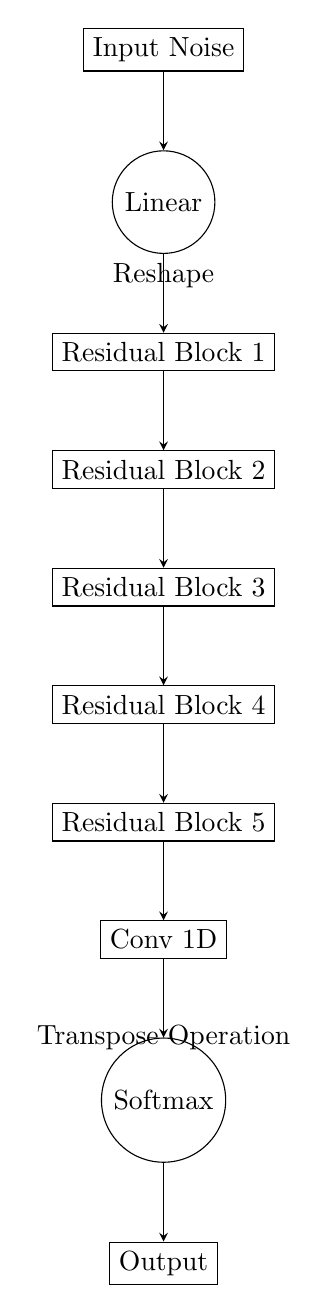
\begin{tikzpicture}
      \node[draw] (input) at (0, 0) {Input Noise};
      \node[draw, circle, below=of input] (linear) {Linear};
      \node[draw, below=of linear] (resblock1) {Residual Block 1};
      \node[draw, below=of resblock1] (resblock2) {Residual Block 2};
      \node[draw, below=of resblock2] (resblock3) {Residual Block 3};
      \node[draw, below=of resblock3] (resblock4) {Residual Block 4};
      \node[draw, below=of resblock4] (resblock5) {Residual Block 5};
      \node[draw, below=of resblock5] (conv1d) {Conv 1D};
      \node[draw, circle, below=of conv1d] (softmax) {Softmax};
      \node[draw, below=of softmax] (output) {Output};
      \draw[-stealth] (input.south) -| (linear.north) node[midway,right] {};
      \draw[-stealth] (linear.south) -| (resblock1.north) node[midway,below] 
      {Reshape};
      \draw[-stealth] (resblock1.south) -| (resblock2.north) node[]{};
      \draw[-stealth] (resblock2.south) -| (resblock3.north) node[]{};
      \draw[-stealth] (resblock3.south) -| (resblock4.north) node[]{};
      \draw[-stealth] (resblock4.south) -| (resblock5.north) node[]{};
      \draw[-stealth] (resblock5.south) -| (conv1d.north) node[]{};
      \draw[-stealth] (conv1d.south) -| (softmax.north) node[]{
        Transpose Operation
      };
      \draw[-stealth] (softmax.south) -| (output.north) node[]{};
    \end{tikzpicture}
    \caption{Generatoriaus neuroninio tinklo sandara.}
  \end{subfigure}
  \hfill
  \begin{subfigure}[b]{0.25\textwidth}
    \centering
    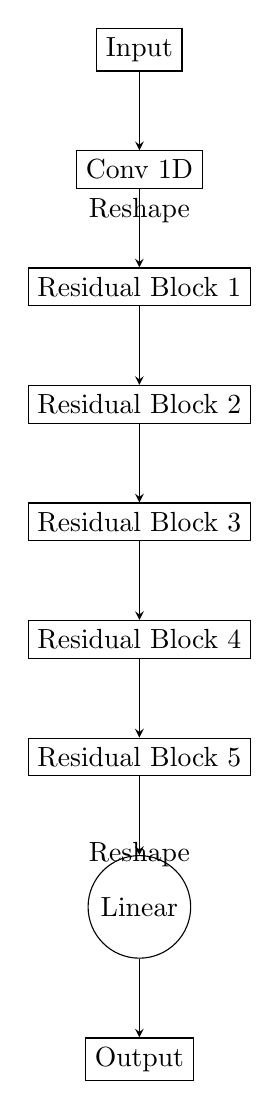
\begin{tikzpicture}
      \node[draw] (input) at (0, 0) {Input};
      \node[draw, below=of input] (conv1d) {Conv 1D};
      \node[draw, below=of conv1d] (resblock1) {Residual Block 1};
      \node[draw, below=of resblock1] (resblock2) {Residual Block 2};
      \node[draw, below=of resblock2] (resblock3) {Residual Block 3};
      \node[draw, below=of resblock3] (resblock4) {Residual Block 4};
      \node[draw, below=of resblock4] (resblock5) {Residual Block 5};
      \node[draw, circle, below=of resblock5] (linear) {Linear};
      \node[draw, below=of linear] (output) {Output};
      \draw[-stealth] (input.south) -| (conv1d.north) node[midway,right] {};
      \draw[-stealth] (conv1d.south) -| (resblock1.north) node[midway,below] 
      {Reshape};
      \draw[-stealth] (resblock1.south) -| (resblock2.north) node[]{};
      \draw[-stealth] (resblock2.south) -| (resblock3.north) node[]{};
      \draw[-stealth] (resblock3.south) -| (resblock4.north) node[]{};
      \draw[-stealth] (resblock4.south) -| (resblock5.north) node[]{};
      \draw[-stealth] (resblock5.south) -| (linear.north) node[]{Reshape};
      \draw[-stealth] (linear.south) -| (output.north) node[]{};
    \end{tikzpicture}
    \caption{Diskriminatoriaus neuroninio tinklo sandara.}
  \end{subfigure}
  \caption{\textquote{PassGAN} metodo neuroniniai tinklai.}
  \label{plot:passganarch}
\end{figure}

\end{document}
